

\chapter{Einleitung}\label{sec:Einleitung}

Das \emph{Semantic Web} erweitert das heutige Web um explizite Bedeutung: Inhalte werden so strukturiert, dass nicht nur Menschen, sondern auch Programme die Semantik verarbeiten und komplexe Aufgaben automatisiert unterstützen können \cite{bernersLee2001}. Dazu werden Informationen maschinenlesbar beschrieben (u.\,a.\ via URIs/IRIs und RDF-Tripeln), sodass Software-Agenten Datenquellen verbinden, Schlussfolgerungen ziehen und Dienste koordinieren können – ohne zentrale Steuerung und im Sinne eines dezentralen, evolvierenden Webs \cite{bernersLee2001}.

Auf dieser Grundlage haben sich \emph{Wissensgraphen} als flexible Datenabstraktion etabliert: Sie verbinden Entitäten und Relationen in einem strukturierbaren, navigierbaren Graphenmodell \cite{hogan2021}. Als Abfragesprache dient \emph{SPARQL}, das graphbasierte Muster formuliert und semantisch interpretierbar macht \cite{w3cSparql11}. Die Komplexität der Syntax stellt jedoch für viele Endnutzer:innen eine Herausforderung dar \cite{perezGutierrezSparql}.

Parallel vergrößern \emph{Large Language Models (LLMs)} den Gestaltungsspielraum natürlicher Schnittstellen. GPT-4 zeigt, dass Modelle natürliche Sprache robust verarbeiten und in anspruchsvollen Benchmarks Leistungsniveaus nahe menschlicher Expert:innen erreichen können – bei bekannten Grenzen wie Halluzinationen und der Notwendigkeit geeigneter Sicherheitsmaßnahmen \cite{openaiGPT42023}. Dies legt nahe, natürliche Sprache als Interface zu RDF-Daten nutzbar zu machen: Benutzer:innen formulieren Aufgaben in Alltagssprache; ein LLM generiert daraus \emph{valide} SPARQL-Operationen.

Für reale, domänenspezifische Wissensgraphen (z.\,B.\ historische Personen, Orte, Organisationen) genügt es jedoch nicht, nur SELECT-Anfragen abzudecken. Gefordert ist die \emph{semantische Bearbeitung} – \textbf{INSERT}, \textbf{DELETE} und \textbf{UPDATE} – mit \emph{Nachvollziehbarkeit} und \emph{Sicherheit}. Dabei ist der \textbf{Datenschutz} zentral: Bei natürlicher Spracheingabe, Prompt-Kontext und beim Logging können personenbezogene Daten betroffen sein; die EU-DSGVO fordert u.\,a.\ Datenminimierung, Zweckbindung, Integrität/Vertraulichkeit und Rechenschaftspflicht \cite{euGDPR2016}. Privacy-by-Design ergibt sich hier u.\,a.\ durch die Beschränkung des Modellkontexts auf \emph{Ontologie statt Instanzdaten} sowie durch Pseudonymisierung und strikte Aufbewahrungsregeln für Query-Logs.

\paragraph{Ziel der Arbeit.}
Diese Arbeit konzipiert, implementiert und evaluiert eine Schnittstelle, die \emph{natürliche Sprache} in \emph{valide SPARQL-Änderungsoperationen} überführt und Datenschutz sowie Nachvollziehbarkeit durchgängig verankert. Kernideen sind:
\begin{enumerate}
\item LLM-gestützte Generierung mit \emph{Ontologie-Kontext} (Klassen/Properties) statt vollständiger Instanzdaten,
\item \emph{Vorschau} und \emph{Erklärung} der betroffenen Tripel,
\item \emph{schrittweise Bestätigung} und \emph{Undo},
\item \emph{Protokollierung} mit Pseudonymisierung und klaren Lösch-/Aufbewahrungsregeln.
\end{enumerate}

\paragraph{Eigene Beiträge.}
Gegenüber bestehenden NL{\textrightarrow}SPARQL-Ansätzen fokussiert diese Arbeit drei miteinander verzahnte Neuerungen:  
(i) ein Ontologie-only-Prompting, das personenbezogene Instanzdaten konsequent aus dem LLM-Kontext heraushält,  
(ii) ein zweistufiger Preview/Execute-Workflow mit bestätigungspflichtigem Token, Explainability und deterministischen Undo-Queries,  
(iii) ein Logging-Konzept, das Pseudonymisierung und Privacy-by-Design-Metadaten (DPV) kombiniert.

Die Architektur und Referenzimplementierung wurden vollständig vom Autor entwickelt und in eine produktionsnahe Entwicklungsumgebung der Pfarrerdatenbank überführt. In der Evaluation (Kapitel~\ref{sec:evaluation}) werden diese Bausteine gemeinsam betrachtet und gegenüber Anforderungen aus Datenschutz, Governance und Usability reflektiert.

\paragraph{Forschungsfragen.}
\begin{description}
\item[RQ1:] Mit welcher Genauigkeit lassen sich natürliche \emph{Änderungsanweisungen} in \emph{syntaktisch valide} und \emph{semantisch korrekte} SPARQL-Operationen (INSERT/DELETE/UPDATE) überführen?
\item[RQ2:] Wie wirken \emph{Privacy-by-Design}-Maßnahmen (Ontologie-Kontext, Pseudonymisierung von Logs) auf Datenschutz, Nachvollziehbarkeit und Nutzbarkeit?
\item[RQ3:] Wie lässt sich die \emph{Benutzbarkeit} (Verständlichkeit von Vorschau, Erklärungen, Undo) theoretisch reflektieren, und wie zeigt sie sich exemplarisch in einem qualitativen Walkthrough?
\end{description}

\paragraph{Struktur der Arbeit.}
Die Arbeit liefert (i) eine \emph{Anforderungsanalyse} für NL{\textrightarrow}SPARQL-Änderungen unter DSGVO-Vorgaben,  
(ii) eine \emph{Architektur} mit Komponenten für Prompting/Parser, Generator, Validator, Executor, Logger und Visualizer,  
(iii) eine \emph{Referenzimplementierung} (Frontend/Backend, SPARQL-Endpoint)  
und (iv) eine \emph{Evaluation} auf einer domänennahen Wissensbasis.

Kapitel~\ref{sec:theorie} fasst zunächst die theoretischen Grundlagen zusammen, darunter RDF, OWL, SPARQL, Large Language Models sowie zentrale Aspekte des Datenschutzes. Anschließend gibt Kapitel~\ref{sec:related-work} einen Überblick über verwandte Arbeiten. Die Anforderungsanalyse und Konzeption der Schnittstelle werden in Kapitel~\ref{sec:konzeption} erläutert, gefolgt von der konkreten Implementierung in Kapitel~\ref{sec:implementierung}. Kapitel~\ref{sec:evaluation} beschreibt die Evaluation der entwickelten Lösung. Abschließend zieht Kapitel~\ref{sec:fazit} ein Fazit und gibt einen Ausblick auf mögliche Weiterentwicklungen.








\chapter{Theoretischer Hintergrund}
\label{sec:theorie}

\section{Grundlagen des Semantic Web}
\label{sec:grundlagen-semantic-web}

\subsection{Motivation und Grundidee}

Das World Wide Web ist allgegenwärtig und wächst stetig; seine Stärken -- hohe Aktualität, globale Verfügbarkeit und niedrige Publikationsschwellen -- gehen zugleich mit Herausforderungen einher: heterogene Formate, fehlende Qualitätssicherung und vor allem eine \emph{mangelnde maschinelle Interpretierbarkeit} von Inhalten \cite{Hitzler}. Suchmaschinen mildern dies mit statistischen Verfahren, bleiben jedoch letztlich stichwort- statt bedeutungsbasiert. 

Die Idee des \emph{Semantic Web} (SW) ist, Informationen \emph{von vornherein} so zu repräsentieren, dass sie von Maschinen verarbeitet, zusammengeführt und logisch erschlossen werden können -- interoperabel durch offene Standards wie RDF, RDFS, OWL und SPARQL \cite{Hitzler,AntoniouVanHarmelen}. Leitgedanke: \emph{Informationen so repräsentieren, dass Maschinen damit in menschlich nützlicher Weise umgehen können} \cite{Hitzler}.


\subsection{Globale Bezeichner: URIs/IRIs und Blank Nodes}

Interoperabilität setzt globale Identifizierbarkeit voraus. RDF verwendet dafür \emph{IRIs} (Internationalized Resource Identifiers) — Unicode-fähige Web-Adressen zur eindeutigen Benennung von Ressourcen und Eigenschaften. IRIs erweitern das URI-Konzept (\emph{Uniform Resource Identifier}), das ursprünglich auf ASCII beschränkt war. In RDF können IRIs an Subjekt-, Prädikat- und Objektpositionen auftreten; alternativ sind Literale als Objekt zulässig. Literale modellieren Basiswerte mit Datentyp (z.\,B.\ \texttt{xsd:decimal}) und optionalem Sprach-Tag. \emph{Blank Nodes} hingegen bezeichnen namenlose Hilfsknoten (nur Subjekt/Objekt) und dienen der Strukturierung, erschweren jedoch Identitätsabgleich und verteilte Abfragen \cite{RDF11Primer,Hitzler}.

\subsection{RDF -- Datenmodell und Serialisierungen}
\label{subsec:rdf}

Das \emph{Resource Description Framework} (RDF) beschreibt Wissen als gerichtete Tripel
\(\langle\)\emph{Subjekt, Prädikat, Objekt}\(\rangle\) und formt daraus Graphen. RDF ist domänenneutral, dezentral kombinierbar und fördert Wiederverwendung: Tripel aus verschiedenen Quellen lassen sich zusammenführen, sofern IRIs konsistent verwendet werden \cite{RDF11Primer,AntoniouVanHarmelen,Hitzler}.

\paragraph{Knotenarten.} (RDF kennt drei Arten von Knoten: (i) IRIs zur Benennung von Ressourcen und Eigenschaften, (ii) Literale als getypte Basiswerte (z.B. Dezimalzahlen oder Strings mit Sprachangabe), sowie (iii) Blank Nodes als namenlose Platzhalter, etwa für strukturierende Zwischenelemente. \cite{RDF11Primer}.

\begin{figure}[h]
\centering
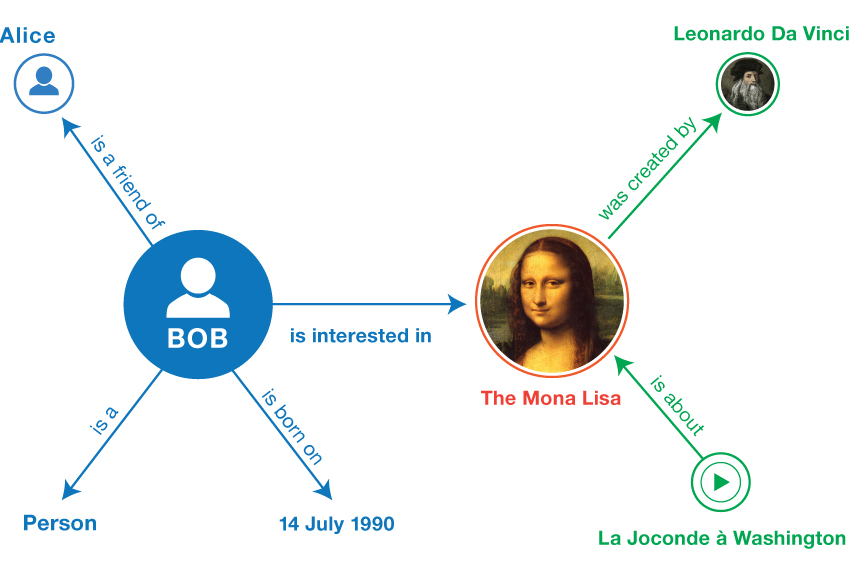
\includegraphics[width=\linewidth]{Abbildungen/example-graph.jpg}
\caption{Beispielhafter Aufbau eines RDF-Graphen.}
\label{fig:example-rdf-graph}
\end{figure}

\footnotetext{Quelle: \url{https://www.w3.org/TR/rdf11-primer/}}

\paragraph{Datensätze und benannte Graphen.} RDF erlaubt die Gruppierung mehrerer Graphen in Datensätzen (\emph{named graphs}) für die Bildung von Teilmengen und die Angabe der Datenherkunft (Provenienz) \cite{RDF11Primer}.

\paragraph{Serialisierungen/Dateiformate.} Für Austausch und Lesbarkeit existieren mehrere Schreibweisen mit gleicher Semantik: \emph{Turtle} (menschlich gut lesbar), \emph{N-Triples/N-Quads} (zeilenbasiert, großskaliger Austausch), \emph{TriG} (Datensätze), \emph{JSON-LD} (JSON-native Einbettung) sowie \emph{RDFa} (Einbettung in HTML) \cite{RDF11Primer}.

\paragraph{Beispiel (Turtle).}\mbox{}\\[-1.5ex]
\begin{lstlisting}
@prefix ex:  <http://example.org/> .
@prefix xsd: <http://www.w3.org/2001/XMLSchema#> .

ex:SemanticWeb a ex:Buch ;
  ex:titel "Semantic Web – Grundlagen"@de ;
  ex:autor ex:Hitzler, ex:Kroetzsch, ex:Rudolph, ex:Sure ;
  ex:preis "42.00"^^xsd:decimal .
\end{lstlisting}

\paragraph{Vokabulare.} RDF selbst legt die \emph{Bedeutung} verwendeter Bezeichner nicht fest. Erst wohldefinierte Vokabulare und Ontologiesprachen präzisieren Semantik -- siehe RDFS/OWL \cite{Hitzler,AntoniouVanHarmelen}.



\subsection{RDFS -- Schematisierung und leichtgewichtige Inferenz}

\emph{RDF Schema} (RDFS) erweitert RDF um Basiskonzepte für Klassen und Eigenschaften, u.\,a.\ \texttt{rdfs:Class}, \texttt{rdf:Property}, Subklassen/Subproperties (\texttt{rdfs:subClassOf}/\texttt{rdfs:subPropertyOf}), sowie \texttt{rdfs:domain}/\texttt{rdfs:range} zur Typisierung von Subjekt/Objekt. Damit lassen sich eigene Vokabulare definieren und einfache Ableitungen (z.\,B.\ Typvererbung) durchführen \cite{RDFS11,Hitzler}.

\paragraph{Beispiel (Turtle).}\mbox{}\\[-1.5ex]
\begin{lstlisting}
ex:Universitaet rdfs:subClassOf ex:Institution .

ex:istVerheiratetMit a rdf:Property ;
  rdfs:domain ex:Person ;
  rdfs:range  ex:Person .

ex:istGluecklichVerheiratetMit
  rdfs:subPropertyOf ex:istVerheiratetMit .
\end{lstlisting}

RDFS ist ein \emph{universelles} Vokabular: Es beschreibt die Semantik der \emph{eigenen Begriffe} eines Domänenvokabulars, nicht die Domäne selbst. Ausdrucksstärke und Inferenz bleiben bewusst einfach und effizient \cite{RDFS11}.

\subsection{OWL~2 -- Ontologien und Schlussfolgern}
\label{subsec:owl}

Komplexere Abhängigkeiten überschreiten die Ausdruckskraft von RDFS. Die \emph{Web Ontology Language} (OWL~2) basiert auf Beschreibungslogiken und bietet reichhaltige Konstruktoren (Schnittmenge, Vereinigung, Komplement), Disjunktheit/Äquivalenz von Klassen, Kardinalitäten sowie Eigenschaften-Charakteristika (symmetrisch, transitiv, funktional etc.). Für verschiedene Praxisanforderungen existieren die OWL-2-Profile EL (für große, tief gestaffelte Hierarchien), QL (für effiziente SQL-basierte Abfragen über große Datenbestände) und RL (für regelbasierte Inferenz/Materialisierung), die garantieren, dass Schlussfolgerungen effizient berechnet werden können \cite{Hitzler,AntoniouVanHarmelen,OWL2Overview}. Die Möglichkeit, Klassen- und Eigenschaftshierarchien zu modellieren, ist entscheidend für kontextsensitives Prompting in dieser Arbeit.

\paragraph{Skizze (RDF/XML-Ausschnitt).}\mbox{}\\[-1.5ex]
\begin{lstlisting}
<owl:Class rdf:about="ex:Professor"/>
<ex:Person rdf:about="ex:RudiStuder"/>
<owl:ObjectProperty rdf:about="ex:arbeitetGernMit"/>
\end{lstlisting}

\subsection{SPARQL~1.1 -- Abfragen über Graphen}
\label{subsec:sparql}

SPARQL ist die standardisierte Abfragesprache für RDF-Daten. Abfragen in SPARQL beruhen auf sogenannten \emph{Graphmustern}: Sie beschreiben Strukturmuster, die im RDF-Graphen gesucht werden sollen. Solche Muster bestehen aus mehreren \emph{Tripelmustern} — das sind Platzhaltervarianten der RDF-Tripel mit Variablen anstelle von konkreten Ressourcen. Tripel- und Graphmuster bilden die Grundlage für SPARQL-Änderungen, wie sie später durch LLMs automatisch generiert werden (Kapitel~\ref{sec:implementierung}). Ein einfaches Tripelmuster wäre z.\,B.\ \texttt{\{ ?person ex:geburtsjahr ?jahr \}}, das nach allen Personen sucht, für die ein Geburtsjahr verzeichnet ist. SPARQL kombiniert mehrere Tripelmuster zu komplexen Mustern mittels Konstrukten wie \texttt{OPTIONAL} (für optionale Teilmuster, ähnlich Left-Outer-Join), \texttt{UNION} (für Alternativen), \texttt{FILTER} (für Bedingungen), sowie \emph{Property Paths}, die eine Navigation über Pfade beliebiger Länge ermöglichen. Zusätzlich stehen Aggregationen, Unterabfragen und Bindungsfunktionen zur Verfügung.
Die Ergebnisform der Abfrage wird durch das Schlüsselwort bestimmt:
\begin{itemize}
  \item \texttt{SELECT} gibt Variablenbindungen als Tabellen zurück,
  \item \texttt{CONSTRUCT} erzeugt neue RDF-Graphen auf Basis eines Zielmusters,
  \item \texttt{ASK} prüft lediglich, ob eine Lösung existiert (Boolean),
  \item \texttt{DESCRIBE} liefert eine systemabhängige Beschreibung von Ressourcen.
\end{itemize}
Zur Steuerung der Ausgabe unterstützen SPARQL-Abfragen Modifikatoren wie \texttt{ORDER BY}, \texttt{LIMIT}/\texttt{OFFSET} (Paginierung) und \texttt{DISTINCT} (Duplikateliminierung) \cite{SPARQL11Overview,Hitzler,AntoniouVanHarmelen}.
Ein Beispiel für eine typische SELECT-Abfrage findet sich weiter unten. Dort wird geprüft, welche Bücher bei einem bestimmten Verlag verlegt wurden; zusätzlich wird (optional) der Autor ermittelt.


\paragraph{Beispiel (SELECT).}\mbox{}\\[-1.5ex]
\begin{lstlisting}
PREFIX ex: <http://example.org/>
SELECT ?titel ?autor
WHERE {
  ?buch ex:verlegtBei <http://springer.com/Verlag> ;
        ex:titel ?titel .
  OPTIONAL { ?buch ex:autor ?autor . }
}
ORDER BY ?titel
\end{lstlisting}

\paragraph{Formale Sicht und Komplexität.}
Die Auswertung basiert auf Graph-Homomorphismen mit \emph{Bag}- und \emph{Set}-Semantik; Sprachkonstrukte wie \texttt{OPTIONAL}, \texttt{UNION} und Filter führen zu nichttrivialen Komplexitätsklassen -- relevant für Optimierung und Systemdesign \cite{perezGutierrezSparql}.

\paragraph{SPARQL-Endpunkte (Definition und Nutzung).}
Ein \emph{SPARQL-Endpunkt} ist ein HTTP-basiertes Web-API, das SPARQL-Anfragen (READ: \texttt{SELECT}/\texttt{ASK}/\texttt{CONSTRUCT}/\texttt{DESCRIBE}) und oft auch Updates (\texttt{INSERT}/\texttt{DELETE}) entgegennimmt und ausführt. Clients senden Queries typischerweise via \texttt{GET} (URL-kodiert) oder \texttt{POST} (Body), Antworten werden als SPARQL-Results (JSON/XML) bzw.\ als RDF-Serialisierung geliefert; Timeouts, Limits und Zugriffskontrolle sind üblich. Ein Endpunkt exponiert damit ein RDF-\emph{Dataset} (Default- und benannte Graphen) über das Web und folgt dem SPARQL-1.1-Protokoll/Service-Description-Modell \cite{SPARQL11Overview}. Ein minimalistisches Beispielaufrufmuster ist:
\begin{lstlisting}[language=bash]
curl -G 'https://example.org/sparql' \
  --data-urlencode 'query=SELECT * WHERE { ?s ?p ?o } LIMIT 10'
\end{lstlisting}

\subsection{Validierung: SHACL}

\emph{SHACL} beschreibt \emph{Shapes} mit Constraints (z.\,B.\ \texttt{sh:minCount}, \texttt{sh:datatype}, \texttt{sh:class}, \texttt{sh:pattern}), gegen die Datengraphen validiert werden; das Ergebnis ist ein Validierungsbericht mit Fokusknoten, Pfad, Ursache und Schweregrad \cite{SHACL12}. In dieser Arbeit dient SHACL als Baustein für frühzeitige Qualitätskontrollen und Policy-Checks; Details folgen im Validierungs-Kapitel.


\subsection{Datenschutz (Brücke)}

Sobald personenbezogene Daten betroffen sind, gelten die EU-DSGVO-Vorgaben (z.\,B.\ Datenminimierung, Zweckbindung, Integrität/Vertraulichkeit, Rechenschaftspflicht) \cite{euGDPR2016}. Wir adressieren dies später durch Privacy-by-Design-Maßnahmen (Ontologie-only-Prompting, Pseudonymisierung, restriktive Logs) und eine entsprechende Ausführungs-/Governance-Pipeline.

\subsection*{Zwischenfazit}

RDF liefert das neutrale Graph-Datenmodell; RDFS und OWL~2 fügen Semantik und Inferenz hinzu. SPARQL~1.1 bietet Abfrage- und Änderungsmechanismen; SHACL ergänzt Validierung. Dieses Fundament ermöglicht es, natürlichsprachliche Anweisungen in \emph{valide} SPARQL-Operationen zu überführen und sie unter Berücksichtigung von Qualität und Datenschutz kontrolliert auszuführen \cite{Hitzler,RDF11Primer,RDFS11,OWL2Overview,SPARQL11Overview,hogan2021,perezGutierrezSparql,SHACL12}.







\section{Vorstellung der Pfarrerdatenbank}
\label{sec:Pfarrerdatenbank}

\subsection{Ziel und Überblick}
Die \emph{Pfarrerdatenbank} (Meta-Pfarrerbuch) vereinheitlicht Metadaten zu evangelischen Pfarrerinnen und Pfarrern aus mehreren regionalen Projekten und stellt sie als verknüpfte, maschinenlesbare RDF-Daten bereit. Der Fokus liegt auf einer konsistenten, quer über Regionen vergleichbaren Erfassung von Personen, ihren Lebensabschnitten (z.,B. Geburt, Ordination, Dienststellen), Orten und Quellen. Die Daten werden in RDF serialisiert und über einen kombinierten SPARQL-Dienst abgefragt; eine Web-UI (\texttt{pfarrerbuch-meta}) nutzt diesen Endpunkt für Suche und Anzeige.

\subsection{Quellen, Vokabular und Umfang}
Die gelieferten Datenquellen liegen regional getrennt als N-Triples vor und werden durch ein projektspezifisches Vokabular ergänzt:
\begin{itemize}
\item \texttt{meta-sachsen.nt.gz} – Sachsen ($\approx$\,825{,}087 Tripel)
\item \texttt{meta-brandenburg.nt.gz} – Brandenburg ($\approx$\,269{,}835 Tripel)
\item \texttt{meta-kps.nt.gz} – Kurland/Piltens/Semgallen u.\,a. ($\approx$\,305{,}450 Tripel)
\item \texttt{vocabulary.nt.gz} – projektspezifisches RDF/RDFS-Vokabular ($\approx$\,3{,}211 Tripel)
\end{itemize}
Für die Bereitstellung wird daraus ein N-Quads-Gesamtdatensatz \texttt{meta-combined.nq.gz} ($\approx$\,1{,}403{,}584 Quads) erzeugt, der vier benannte Graphen enthält:
\path{/data/graphs/brandenburg}, \path{/data/graphs/kps}, \path{/data/graphs/sachsen} und \path{/vocabulary\#}.

Das Vokabular ist unter
\url{http://meta-pfarrerbuch.evangelische-archive.de/vocabulary\#} bereitgestellt. Zentrale Klassen/Properties, die auch in den Beispielen unten verwendet werden:
\begin{itemize}
\item \textbf{Klassen:} \texttt{pfb:Person}, \texttt{pfb:Lebensabschnitt}, \texttt{pfb:Geburt}, \texttt{pfb:Ort}.
\item \textbf{Properties:} \texttt{pfb:vorname}, \texttt{pfb:nachname}, \texttt{pfb:hatLebensabschnitt}, \texttt{pfb:jahr}, \texttt{pfb:datum}, \texttt{pfb:hatOrt}, \texttt{pfb:derivedFrom}.
\end{itemize}

\subsection{Build‐/Publikationsprozess}
Der Build-Schritt erfolgt skriptgestützt (\texttt{generate-combined.sh}). Die Dienste werden in \texttt{config.ttl} beschrieben: Neben getrennten Services für \emph{sachsen}, \emph{brandenburg}, \emph{kps} und \emph{vocabulary} ist ein virtueller Service \texttt{combined} definiert, der alle benannten Graphen als einen SPARQL-Endpunkt zusammenführt. Die Web-UI \texttt{pfarrerbuch-meta} (GitHub: \texttt{pcp-on-web/pfarrerbuch-meta}\footnote{Internes GitHub-Repository; der Zugriff auf \texttt{pcp-on-web/pfarrerbuch-meta} ist projektintern geregelt.}) fragt diesen Endpunkt und rendert die Daten in einer nutzerfreundlichen Oberfläche.

\subsection{Datenmodell}
\textbf{Personen} (\texttt{pfb:Person}) tragen unter anderem \texttt{pfb:vorname} und \texttt{pfb:nachname}. \textbf{Lebensabschnitte}
(\texttt{pfb:Lebensabschnitt}) hängen über \texttt{pfb:hatLebensabschnitt} an Personen und sind typisiert
(z.,B. \texttt{pfb:Geburt}). Für Ereignisse stehen die zeitlichen Felder \texttt{pfb:jahr}/\texttt{pfb:datum} sowie Ortsbezüge
(\texttt{pfb:hatOrt}) bereit. Provenienz kann über \texttt{pfb:derivedFrom} referenziert werden. Das Modell bildet so einen gut querverknüpften RDF-Graph mit klaren regionalen Grenzen (benannte Graphen), der sowohl Gesamtabfragen als auch gezielte Regionalabfragen erlaubt.

\subsection{Architektur}
\begin{figure}[h]
\centering
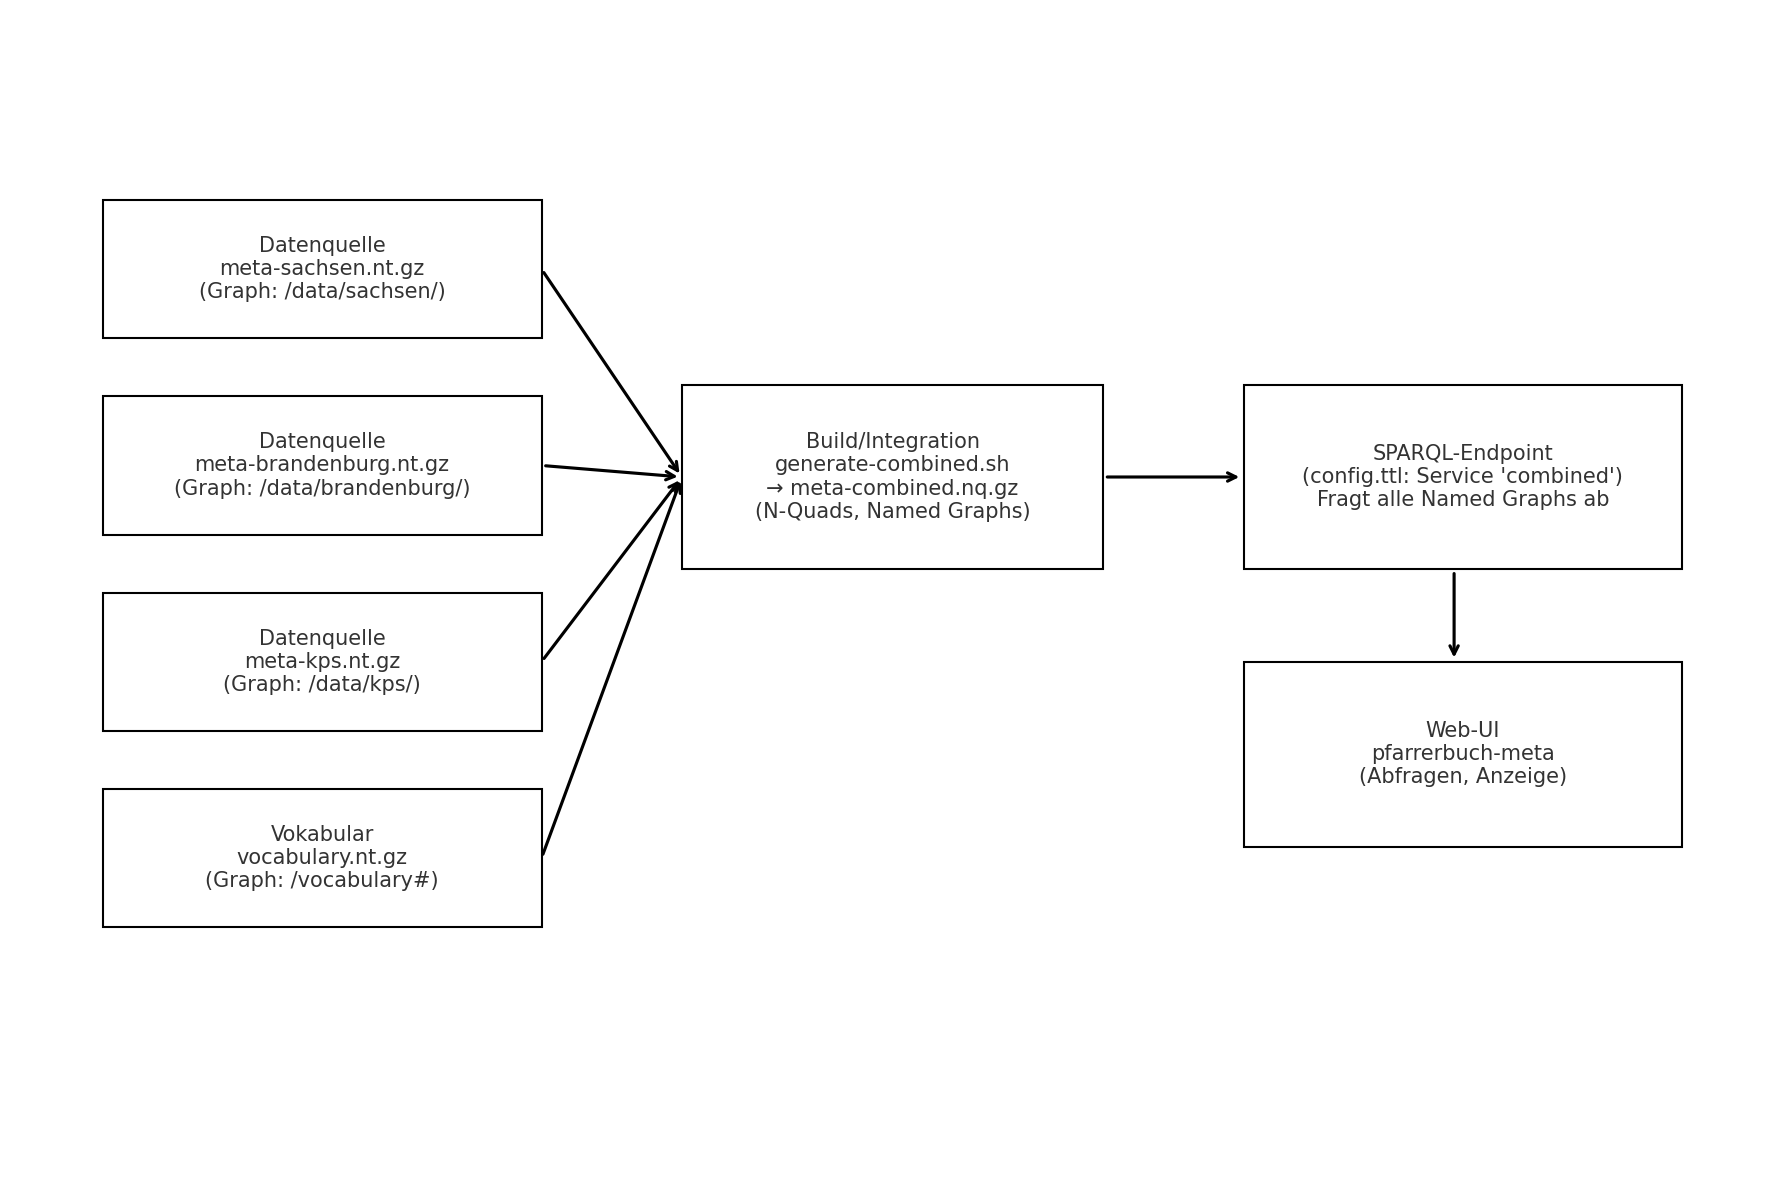
\includegraphics[width=\linewidth]{Abbildungen/Aufbau_Pfarrerdatenbank.jpg}
\caption{Architektur der Pfarrerdatenbank (Quellen $\rightarrow$ Build/Integration $\rightarrow$ kombinierter SPARQL-Dienst $\rightarrow$ Web-UI).}
\label{fig:pfarrer-architektur}
\end{figure}

\noindent Die Abbildung zeigt die vier Bausteine: (1) regionale N-Triples und Vokabular, (2) Skriptbasierter Merge nach N-Quads
(\texttt{meta-combined.nq.gz}) mit benannten Graphen, (3) SPARQL-Endpoint \emph{combined} aus \texttt{config.ttl}, (4) die Web-UI.

\subsection{SPARQL-Beispiele}
\noindent Präfixe (für alle Beispiele):
\begin{verbatim}
PREFIX pfb: <http://meta-pfarrerbuch.evangelische-archive.de/vocabulary#>

PREFIX rdf: <http://www.w3.org/1999/02/22-rdf-syntax-ns#>

PREFIX rdfs: <http://www.w3.org/2000/01/rdf-schema#>

PREFIX xsd: <http://www.w3.org/2001/XMLSchema#>

\end{verbatim}

\paragraph{(a) Anzahl Personen gesamt und pro Graph}
\begin{verbatim}
SELECT (COUNT(DISTINCT ?p) AS ?personenGesamt) WHERE {
  GRAPH ?g { ?p rdf:type pfb:Pfarrer-in . }
}

SELECT ?g (COUNT(DISTINCT ?p) AS ?anzahl) WHERE {
  GRAPH ?g { ?p rdf:type pfb:Pfarrer-in . }
} GROUP BY ?g
\end{verbatim}

\paragraph{(b) Personen mit Name und Geburtsjahr}
\begin{verbatim}
SELECT ?p ?nach ?vor ?jahr WHERE {
  GRAPH ?g {
    ?p rdf:type pfb:Pfarrer-in ;
       pfb:nachname ?nach ;
       pfb:vorname ?vor ;
       pfb:hatLebensabschnitt ?la .
    ?la rdf:type pfb:Geburt .
    OPTIONAL { ?la pfb:jahr ?jahr }
  }
} LIMIT 50
\end{verbatim}

\paragraph{(c) Auf Sachsen eingrenzen (benannter Graph)}
\begin{verbatim}
SELECT ?p ?nach ?vor WHERE {
  GRAPH <http://meta-pfarrerbuch.evangelische-archive.de/data/sachsen/> {
    ?p rdf:type pfb:Pfarrer-in ;
       pfb:nachname ?nach ;
       pfb:vorname ?vor .
  }
} LIMIT 50
\end{verbatim}

\paragraph{(d) Geburtsort (sofern vorhanden)}
\begin{verbatim}
SELECT ?p ?nach ?vor ?ort WHERE {
  GRAPH ?g {
    ?p rdf:type pfb:Pfarrer-in ;
       pfb:nachname ?nach ;
       pfb:vorname ?vor ;
       pfb:hatLebensabschnitt ?la .
    ?la rdf:type pfb:Geburt .
    OPTIONAL { ?la pfb:hatOrt ?ort }
  }
} LIMIT 50
\end{verbatim}

\subsection{Fazit}
Die Pfarrerdatenbank stellt einen integrierten RDF-Wissensgraph über mehrere Regionen bereit. Das eigene Vokabular und die klare Trennung per benannten Graphen ermöglichen sowohl aggregierte Queries als auch präzise Regionalsichten. Über den kombinierten SPARQL-Endpunkt versorgt die Web-UI Forschende und die interessierte Öffentlichkeit mit konsistenten, zitierfähigen Daten.








\section{Einführung in Large Language Models}
\label{sec:llm}

\subsection{Einordnung und Motivation}

Große Sprachmodelle (Large Language Models, LLMs) sind tiefneuronale Netze, die auf umfangreichen Textkorpora vortrainiert werden, um die Struktur, Logik und semantischen Muster natürlicher Sprache zu erfassen. Ziel ist in der Regel die Prädiktion des nächsten Tokens $x_t$ gegeben einer Sequenz vorheriger Tokens $x_{<t}$, formal als Wahrscheinlichkeitsverteilung $p(x_t \mid x_{<t})$ modelliert. Dies bildet die Grundlage für Anwendungen wie Textgenerierung, Klassifikation, Übersetzung und Dialogführung.

Im Unterschied zu früheren Systemen basiert der aktuelle Stand der Technik auf der \emph{Transformer}-Architektur \cite{vaswani2017attention}, die durch (i) massive Skalierung von Modell-, Daten- und Rechenressourcen, (ii) effektive Prompting-Methoden für In-Context-Lernen \cite{brown2020language,wei2022chain}, (iii) externe Tool-Nutzung \cite{yao2023react}, sowie (iv) Ausrichtung durch Reinforcement Learning from Human Feedback (RLHF) \cite{ouyang2022training} eine bisher unerreichte Leistungsbreite zeigt.

Dieses Kapitel liefert eine architektonische und methodische Grundlage, erläutert die zentralen Paradigmen (CoT, ReAct, RAG, RLHF), und diskutiert relevante Aspekte zu Datenschutz, Sicherheit und strukturierter Ausgabe (SPARQL). Die behandelten Konzepte werden im weiteren Verlauf praktisch umgesetzt.

\subsection{Transformer-Grundlagen}

\subsubsection{Self-Attention}

Der Transformer ersetzt rekurrente und konvolutionale Strukturen durch einen \emph{Self-Attention}-Mechanismus. Für eine Token-Repräsentation $X \in \mathbb{R}^{n \times d}$ werden Projektionsmatrizen $W_Q$, $W_K$, $W_V$ verwendet, um Queries, Keys und Values zu berechnen: $Q = XW_Q$, $K = XW_K$, $V = XW_V$. Die Ausgabe der Attention lautet:

\[
\mathrm{Attention}(Q,K,V) = \mathrm{softmax}\left( \frac{QK^\top}{\sqrt{d_k}} \right) V
\]

Mehrere Köpfe (\emph{multi-head}) erlauben parallele Fokussierung auf verschiedene Beziehungsmuster. Positionsinformationen werden über (gelernte oder sinusoidale) \emph{Positional Encodings} integriert.

\subsubsection{Architekturvarianten}

Transformer-Modelle treten in zwei Varianten auf:

\begin{itemize}
    \item \textbf{Encoder–Decoder}: für Aufgaben mit Eingabe–Ausgabe-Paaren, z.\,B.\ T5.
    \item \textbf{Decoder-only}: modellieren autoregressiv $p(x_t \mid x_{<t})$, etwa GPT \cite{brown2020language}.
\end{itemize}

Decoder-only-Modelle dominieren bei generativem Prompting. Ein Nachteil ist die quadratische Rechenkomplexität der Attention ($\mathcal{O}(n^2)$); sparsere Varianten verbessern Skalierbarkeit.

\subsubsection{Vortraining: Ziel, Daten, Tokenisierung}

Der Standardansatz ist \emph{Causal Language Modeling} (CLM), oft mit Byte-Pair-Encoding oder Unigram-Tokenisierung. Trainingsdaten umfassen deduplizierte Webkorpora (Common Crawl, Wikipedia, Bücher), wobei Filterregeln Qualität und Datenschutzrisiken (PII) adressieren \cite{brown2020language}.

\subsection{Dekodierung und Textqualität}

\subsubsection{Sampling-Verfahren}

Deterministische Verfahren (Greedy, Beam Search) neigen zu Wiederholungen. Stochastische Methoden wie \emph{Top-$k$ Sampling} und \emph{Nucleus Sampling} (Top-$p$) erzeugen variantenreichere und natürlichere Texte \cite{holtzman2020curious}.

\subsubsection{Neural Text Degeneration}

Als \emph{Degeneration} wird die Tendenz zu repetitiven oder belanglosen Ausgaben bezeichnet. Sie entsteht bei rein likelihooderzeugtem Text. Kalibriertes Sampling, Längen- und Wiederholungskontrollen sowie temperaturbasiertes Sampling wirken dem entgegen.

\subsection{In-Context-Lernen und skalierende Fähigkeiten}

Große Modelle wie GPT-3 \cite{brown2020language} demonstrieren, dass allein durch geschickt formulierte Prompts (ohne Feintuning) Aufgaben gelöst werden können (Zero-/Few-Shot Learning). Prompt-Strategien umfassen:

\begin{itemize}
    \item \textbf{Instruktionsprompting}: Aufgabenbeschreibung in natürlicher Sprache.
    \item \textbf{Few-Shot-Prompting}: Einbindung annotierter Beispiele.
    \item \textbf{Formatvorgaben}: Strukturierte Output-Anweisungen (z.\,B.\ JSON, SPARQL).
\end{itemize}

Leistungszuwächse entstehen insbesondere bei wachsender Modellgröße und Kontexttiefe.

\subsection{Chain-of-Thought (CoT)}

\emph{Chain-of-Thought} erweitert Prompts um explizite Zwischenschritte (Rationale), um komplexe Aufgaben wie Rechnen, logisches Schließen oder Fragebeantwortung zu lösen \cite{wei2022chain}. Koherenz, Konsistenz und Nachvollziehbarkeit steigen; zudem hilft \emph{Self-Consistency} durch Mehrfachsampling und Mehrheitsentscheid.

\paragraph{Grenzen:} CoT ist empfindlich gegenüber Promptformulierung, skaliert schlecht bei kleineren Modellen und kann zu halluzinierten Erklärungen führen.

\subsection{Reason + Act (ReAct): Tool-Nutzung mit LLMs}

\emph{ReAct} kombiniert sprachliche Überlegungen mit externen Aktionen (z.\,B.\ Suche, Kalkulation, SPARQL-Abfragen). Der Ablauf folgt dem Muster:

\texttt{Thought $\rightarrow$ Action $\rightarrow$ Observation $\rightarrow$ Thought ...}

Dies erhöht Genauigkeit, Transparenz und Reduktion von Halluzinationen \cite{yao2023react}. ReAct ist insbesondere für wissensintensive Aufgaben geeignet.

\subsection{Instruction Tuning und RLHF}

\subsubsection{Hintergrund und Pipeline}

Zur besseren Nutzbarkeit werden LLMs auf instruktionsbezogene Daten (z.\,B.\ „Übersetze folgenden Satz...“) per Supervised Fine-Tuning (SFT) angepasst. Anschließend wird ein Belohnungsmodell auf menschliche Präferenzen trainiert, welches wiederum über Reinforcement Learning (meist PPO) optimiert wird \cite{ouyang2022training}.

\begin{enumerate}
    \item \textbf{SFT:} Überwachtes Feintuning auf Beispielanfragen.
    \item \textbf{Reward Modeling:} Menschen bewerten Antwortpaare.
    \item \textbf{RL (PPO):} Modell wird gegen das Belohnungsmodell optimiert.
\end{enumerate}

\paragraph{Begriff: Alignment Tax}

Unter \emph{Alignment Tax} versteht man Leistungseinbußen durch Ausrichtung auf erwünschtes Verhalten (z.\,B.\ geringere Kreativität oder „Übervorsicht“). PPO-PTX (eine Mischung aus RLHF und Pretraining) kann diesen Effekt abmildern.

\subsection{Wissensintensive Aufgaben: RAG und KG-QA}

\subsubsection{Retrieval-Augmented Generation (RAG)}

RAG kombiniert ein Sprachmodell mit einer externen Wissensquelle. Der Ablauf:

\begin{enumerate}
    \item Formulierung der Anfrage
    \item Retrieval passender Dokumente (BM25, DPR, ColBERT)
    \item Verknüpfung mit der Generierung (Late/Joint Fusion)
\end{enumerate}

Vorteile: geringere Halluzinationsrate, aktuellere Fakten, verbesserte Attribution \cite{lewis2020rag}.

\subsubsection{Knowledge Graph QA (KG-QA)}

In Aufgaben wie LC-QuAD~2.0 \cite{dubey2019lcquad2} generieren Modelle SPARQL-Abfragen über Wikidata/DBpedia. Prompting-Techniken fördern dabei „Schema-Ahnung“, also Wissen über Ontologien und Relationen. Alternativ wird ein logisches Zwischenformat erzeugt und dann übersetzt.

\subsection{Strukturierte Ausgaben (SPARQL/JSON)}

LLMs erzeugen standardmäßig Freitext. Für viele Anwendungen (z.\,B.\ SPARQL-Updates) sind aber strukturierte Ausgaben nötig. Drei Methoden unterstützen dies:

\begin{itemize}
    \item \textbf{Schema-Prompting}: Formatvorgaben und Beispiele
    \item \textbf{Constrained Decoding}: Nutzung von Grammatik oder JSON-Schema
    \item \textbf{Reward-Modellierung}: Bestrafung ungültiger Ausgaben im Training \cite{cong2023schema}
\end{itemize}

Für diese Arbeit ist dies entscheidend, um valide, maschineninterpretierbare Ausgaben zu generieren.

\subsection{Sicherheit, Datenschutz und verantwortungsvolle Nutzung}

\subsubsection{Halluzinationen}

Als \emph{Halluzinationen} gelten plausible, aber faktisch falsche Aussagen. Ursachen sind fehlende Evidenz, übergeneralisierte Wahrscheinlichkeitsverteilungen oder aggressive Sampling-Verfahren. Gegenmaßnahmen umfassen ReAct, RAG, konservatives Sampling und Nachverifikation.

\subsubsection{Extraktion von Trainingsdaten}

Studien wie \cite{carlini2021extracting} zeigen, dass seltene Trainingsdaten (z.\,B.\ PII) durch gezielte Prompts reproduziert werden können. Ursachen sind Overfitting, Deduplikationsfehler und unsichere Samplingstrategien.

\subsubsection{Differential Privacy (DP)}

DP-SGD \cite{abadi2016deep} reduziert den Einfluss einzelner Trainingsbeispiele durch Rauschaddition im Gradienten. Es bietet formale Garantien ($\varepsilon$, $\delta$), ist aber mit Genauigkeitseinbußen verbunden. Praktisch vor allem bei kleinen Modellen oder Retrievern relevant.

\subsection{Evaluierung}

\subsubsection{Automatisiert vs. menschlich}

Perplexity misst Sprachflüssigkeit, jedoch nicht Aufgabeerfüllung. Für letzteres eignen sich Metriken wie:

\begin{itemize}
    \item \textbf{Exact Match (EM)}, \textbf{F1-Score}
    \item \textbf{ROUGE}, \textbf{Accuracy}
    \item \textbf{Menschliche Präferenzbewertungen}: Hilfsbereitschaft, Wahrhaftigkeit, Harmlosigkeit
\end{itemize}

\subsubsection{Spezifika für Reasoning}

Bei CoT und ReAct zählen nicht nur Antworten, sondern auch Zwischenschritte. Bewertet werden sollte:

\begin{itemize}
    \item \textbf{Korrektheit} und \textbf{Kohärenz} der Rationales
    \item \textbf{Zitierbarkeit} bzw. Belegbarkeit
    \item \textbf{Selbstkonsistenz} über multiple Sampling-Runs
\end{itemize}

\subsection{Grenzen und Herausforderungen}

\begin{itemize}
    \item \textbf{Skalierungskosten}: Rechenaufwand und Energieverbrauch steigen stark.
    \item \textbf{Kontextlängen}: Quadratische Attention limitiert Eingabelänge; Long-Context-Methoden (FlashAttention, Reformer) sind aktiv in Entwicklung.
    \item \textbf{Bias und Robustheit}: Fehlende Datenvielfalt erzeugt soziale Verzerrungen.
    \item \textbf{Erklärbarkeit}: Begründungen sind nicht gleichzusetzen mit innerer Modelllogik – aber nützlich zur Auditierbarkeit.
\end{itemize}

\subsection{Praxisbausteine}

Für die in dieser Arbeit entwickelte Pipeline genügen modulare Prompt-Templates mit:

\begin{itemize}
    \item Rollenbeschreibung (z.\,B.\ „Du bist ein SPARQL-Generator...“)
    \item Format-Constraints (SPARQL-Block, JSON-Schema)
    \item Optional: Tool-Aktionen im ReAct-Stil (SPARQL, Validator, Undo)
\end{itemize}

Entscheidend ist die Integration mit Validierung, Logging und Datenschutzmaßnahmen.

\subsection{Zusammenfassung}

LLMs verbinden skalierte Transformer-Architekturen mit Prompting, Tool-Nutzung und Ausrichtungstechniken zu universellen Sprachschnittstellen. Chain-of-Thought, ReAct und RAG verbessern reasoningintensive Aufgaben, während SPARQL-Generierung strukturierte Interaktion ermöglicht. Datenschutztechniken wie Differential Privacy und kontrollierte Dekodierung sind entscheidend für den sicheren Einsatz in sensiblen Kontexten. Dieses Fundament wird im weiteren Verlauf praktisch umgesetzt.












\section{Prompt-Programmierung und Few-Shot Learning}
\label{sec:prompting}

\subsection{Paradigmenwechsel: Von Fine-Tuning zu Prompt-Programmierung}

Mit dem Aufstieg großer Sprachmodelle (Large Language Models, LLMs) hat sich ein grundlegender Paradigmenwechsel vollzogen: Statt jede NLP-Aufgabe mit eigenen Modellen via \emph{Fine-Tuning} zu trainieren, werden heute generische, vortrainierte Modelle per Texteingabe (\emph{Prompt}) für Aufgaben aktiviert. Während klassische Verfahren die bedingte Wahrscheinlichkeit einer Zielantwort \(P(y \mid x; \theta)\) lernen, nutzt das Prompting die Textwahrscheinlichkeit \(P(x; \theta)\), indem Aufgaben sprachlich umformuliert werden \cite{liu2023survey}.

Diese Denkweise – \emph{Pre-Train, Prompt, Predict} – bringt drei entscheidende Vorteile:
\begin{itemize}
  \item Nutzung großer Rohtextkorpora für universelles Vortraining,
  \item effektives Zero- und Few-Shot-Lernen ohne Labeldaten,
  \item schnelle Anpassung ohne Modellanpassung, nur durch Prompt-Formulierung.
\end{itemize}

\subsection{Grundlagen: Was ist ein Prompt?}

Ein Prompt ist eine natürlichsprachliche Eingabe, die dem Modell eine Aufgabe beschreibt. Beispiele:
\begin{itemize}
  \item \emph{Klassifikation:} „Ist der folgende Tweet positiv oder negativ? ‘Ich liebe dieses Buch.’“
  \item \emph{KGQA:} „Wie viele Mitarbeiter hat die Firma, deren CEO Tim Cook ist?“
\end{itemize}

Ziel ist es, mit möglichst wenig Beispielen (\emph{Few-Shot}) und ohne explizite Modelländerung valide und nachvollziehbare Antworten zu erzeugen.

\subsection{Formen und Bausteine des Promptings}

\subsubsection{Prompt-Formen: Prefix, Cloze und mehr}

Die Struktur eines Prompts beeinflusst das Antwortverhalten stark. Wichtige Typen:
\begin{itemize}
  \item \textbf{Prefix-Prompts:} Für autoregressive Modelle (z.\,B. GPT). Diese sagen das nächste Token basierend auf dem bisherigen Kontext voraus.
  \item \textbf{Cloze-Prompts:} Für maskierte Modelle (z.\,B. BERT). Hier wird ein Token in der Mitte maskiert, z.\,B.: „Paris ist die Hauptstadt von [MASK].“
  \item \textbf{Mehrfacheingaben:} Aufgaben mit mehreren Inputkomponenten (z.\,B. Satzpaare für Entailment).
\end{itemize}

\subsubsection{Prompt-Template-Engineering}

Die Gestaltung dieser Prompts kann manuell oder automatisiert erfolgen:
\begin{itemize}
  \item \textbf{Diskrete Prompts:} Sprachlich formulierte Templates – manuell geschrieben oder aus Daten abgeleitet (z.\,B. durch Paraphrasierung oder Suche mit Hilfe von seq2seq-Modellen, die Eingabetexte in Prompt-Vorlagen übersetzen).
  \item \textbf{Gradientenbasierte Suche:} Optimierung von Prompt-Templates auf Basis von Modellgradienten (z.\,B. durch differentielles Scoring vieler Varianten).
  \item \textbf{Kontinuierliche („Soft“) Prompts:} Anstelle von Text werden spezielle Einbettungsvektoren trainiert, z.\,B. beim Prefix-Tuning. Diese sind nicht mehr für Menschen lesbar, aber effizient zu optimieren.
\end{itemize}

\subsubsection{Prompt-Answer-Engineering}

Neben dem Prompt selbst ist auch die Ausgestaltung des Antwortraums entscheidend:
\begin{itemize}
  \item \textbf{Antwortformate:} Einzeltoken (z.\,B. „Ja“/„Nein“), Textspannen (mehrere Tokens) oder ganze Sätze.
  \item \textbf{Verbalizer:} Bei Klassifikation wird eine Antwort z.\,B. auf „positiv“/„negativ“ gemappt.
  \item \textbf{Kontrollierte Antwortmengen:} Vorab definierte Auswahlfelder oder strukturierte Formate (z.\,B. SPARQL, JSON).
\end{itemize}

\subsubsection{Mehrfach-Prompts, Kontext und Struktur}

Leistung und Robustheit steigen durch:
\begin{itemize}
  \item \textbf{Prompt-Ensembling:} Mehrere Varianten eines Prompts werden parallel verwendet, Ergebnisse z.\,B. gemittelt oder per Mehrheitsvotum aggregiert.
  \item \textbf{Prompt-Augmentation:} Mehrere Beispiele im Promptkontext (\emph{In-Context Learning}).
  \item \textbf{Prompt-Komposition:} Kombination mehrerer Unterprompts.
  \item \textbf{Dekomposition:} Zerlegung komplexer Aufgaben in Teilaufgaben mit separaten Prompts.
\end{itemize}

\subsection{Reasoning-Techniken: CoT und Self-Consistency}

\subsubsection{Chain-of-Thought (CoT)}

CoT erweitert Few-Shot-Prompts um erklärende Zwischenschritte. Statt nur die Antwort zu nennen, wird die Lösung in logische Teilschritte aufgeteilt:

\emph{Beispiel:}  
„Wie viele Beine haben drei Hunde?“  
→ „Ein Hund hat vier Beine. Drei Hunde haben \(3 \times 4 = 12\) Beine.“

Diese Technik zeigt besonders bei großen Modellen >100B Parameter) emergente Denkfähigkeiten \cite{wei2022cot}.

\subsubsection{Self-Consistency}

Hier wird die gleiche Frage mehrfach beantwortet (z.\,B. 5–10 Samples) und dann die häufigste oder plausibelste Antwort gewählt. Dies erhöht Genauigkeit und Robustheit – besonders bei offenen Fragen \cite{wang2022selfconsistency}.

\subsubsection{Kalibrierung zur Korrektur von Verzerrungen}

Antworten von LLMs können durch irrelevante Faktoren verzerrt werden (z.\,B. Reihenfolge der Beispiele). Die \emph{kontextuelle Kalibrierung} reduziert solche Effekte, indem z.\,B. zuerst mit neutralen Eingaben wie „N/A“ die Modellverzerrung geschätzt und dann kompensiert wird \cite{zhao2021calibrate}.

\subsection{Wissensintensive Aufgaben: Prompting für KGQA und SPARQL}

\subsubsection{Text-zu-SPARQL als strukturierte Alternative}

Bei \emph{Knowledge Graph Question Answering (KGQA)} ist es häufig sinnvoller, statt Freitext direkt strukturierte Abfragen (z.\,B. SPARQL) zu generieren. Diese sind ausführbar und überprüfbar. Studien zeigen: Text-zu-SPARQL ist robuster und halluziniert seltener als reine Freitextausgaben \cite{avila2024autokgqagpt}.

\subsubsection{T-Box, A-Box und Fragmentierung}

Für präzise Abfragen ist eine Kontextbegrenzung entscheidend. Dazu wird der übergebene RDF-Graph fragmentiert und durch:
\begin{itemize}
  \item \textbf{T-Box (Terminologie):} Schema mit Klassen und Relationen,
  \item \textbf{A-Box (Assertionen):} konkrete Fakten/Instanzen,
\end{itemize}
strukturiert übergeben. Prompting bezieht sich dann nur auf relevante Teile. Templates sollten \texttt{OPTIONAL}-Properties, Namespace-Präfixe und stringbasierte Filter (mit \texttt{regex}) korrekt einbinden.

\subsection{Praxismodell: Prompting mit DSPy}

DSPy abstrahiert LLM-Aufrufe über deklarative Module (\texttt{Predict}, \texttt{ReAct}, \texttt{ChainOfThought}), sogenannte \emph{Signaturen} und einen \emph{Teleprompter}, der automatisch Demonstrationen und Hyperparameter optimiert \cite{khattab2023dspy}. Studien zeigen, dass damit robuste Pipelines mit weniger manuellem Aufwand erstellt werden können. Für diese Arbeit wird DSPy als Option erwähnt, jedoch nicht konkret implementiert.

\subsection{Best Practices und Herausforderungen}

\subsubsection*{Offene Herausforderungen}
\begin{itemize}
  \item Generalisierbarkeit über Modellfamilien und -größen ist begrenzt.
  \item Prompt-Stabilität leidet unter Reihenfolgeeffekten und Formatvarianten.
  \item Prompting strukturierter Aufgaben (Tabellen, Graphen) ist weiterhin anspruchsvoll.
\end{itemize}

\subsubsection*{Empfohlene Strategien}
\begin{enumerate}
  \item Klare Aufgabenbeschreibung → geeigneter Prompttyp (Prefix/Cloze).
  \item Repräsentative Demonstrationen + Kontextkalibrierung zur Stabilisierung.
  \item CoT + Self-Consistency für komplexe Denkaufgaben.
  \item Für KGQA: Text-zu-SPARQL mit Fragmentierung und Schema-Prompts.
  \item DSPy als Alternative für modulare, robuste Prompt-Ketten.
\end{enumerate}

\subsection{Fazit}

Prompting hat sich als zentrale Technik zur effektiven Nutzung von LLMs ohne Fine-Tuning etabliert. Durch präzises Template- und Answer-Design, In-Context-Beispiele, CoT, Self-Consistency und Kalibrierung lassen sich leistungsfähige Systeme bauen. Besonders in wissensintensiven Anwendungen wie SPARQL-Generierung bietet Prompting eine präzise, strukturierte und skalierbare Lösung. Konzepte wie DSPy ermöglichen zusätzlich automatisierte Optimierung und bessere Reproduzierbarkeit.











\section{Query-Validierung und Explainability im RDF/SPARQL-Stack}
\label{chap:Query-validation-explainability}

\subsection{Motivation}
RDF, RDFS und OWL spezifizieren vor allem die \emph{Struktur} von Wissensgraphen. Für den Einsatz von automatisch generierten SPARQL-Queries – etwa durch LLMs – genügt dies nicht. Notwendig sind zusätzlich:
\begin{itemize}
\item \textbf{Validierung} gegen modellierte Erwartungen (Constraints),
\item \textbf{Erklärbarkeit} von Query-Ergebnissen und fehlenden Antworten,
\item \textbf{robuste OPTIONAL-Nutzung} zur Erzeugung teilweiser Antworten ohne unerwünschte Komplexität.
\end{itemize}
Dieses Kapitel stellt drei komplementäre Ansätze vor: SPIN als mechanismusnahe Sprache zur Validierung und Inferenz \cite{spin-w3c}, \emph{schwach gut konzipierte} SPARQL-Muster zur sicheren Verwendung von \texttt{OPTIONAL} \cite{kaminski-kostylev-beyond-well-designed} und Provenienzmodelle zur Erklärung von Query-Ergebnissen \cite{green-provenance-semirings,herschel-why-why-not,herschel-survey}.

\subsection{Validierung mit SPIN}

\subsubsection{Kernprinzip}
SPIN (SPARQL Inferencing Notation) beschreibt SPARQL-Queries selbst als RDF-Tripel und ermöglicht deren direkte Verknüpfung mit Klasseninstanzen. Dabei sind vor allem folgende Prädikate zentral:
\begin{itemize}
\item \texttt{spin:constraint}: definiert Bedingungen, die Instanzen erfüllen müssen (z.\,B. mit \texttt{ASK}- oder \texttt{CONSTRUCT}-Abfragen),
\item \texttt{spin:rule}: erlaubt inferenzielle Regeln auf Basis von \texttt{CONSTRUCT} oder \texttt{UPDATE},
\item \texttt{spin:constructor}: initialisiert Instanzen mit Standardwerten.
\end{itemize}
SPIN-Abfragen binden die Variable \texttt{?this} im Klassenkontext; Vererbung erfolgt entlang der \texttt{rdfs:subClassOf}-Hierarchie. Für Optimierungen kann \texttt{spin:thisUnbound} genutzt werden, falls die Abfrage selbst \texttt{?this} bindet \cite{spin-w3c}.

\subsubsection{Fehlermeldungen und Korrekturvorschläge}
\texttt{CONSTRUCT}-Constraints können Verletzungen als \texttt{spin:ConstraintViolation} materialisieren. Diese enthalten typischerweise:
\begin{itemize}
\item \texttt{rdfs:label} zur Beschreibung des Fehlers,
\item \texttt{spin:violationRoot} als referenzierte Instanz,
\item \texttt{spin:violationPath} zur betroffenen Eigenschaft,
\item \texttt{spin:fix} mit optionaler \texttt{UpdateTemplate}-Anweisung zur Behebung.
\end{itemize}

\subsubsection{Beispiel}
\begin{lstlisting}[language=turtle,basicstyle=\ttfamily\small,caption={SPIN-Constraint: Quadrat konsistent halten},label={lst:spin-constraint}]
@prefix ex:   <http://example.org/> .
@prefix spin: <http://spinrdf.org/spin#> .
@prefix sp:   <http://spinrdf.org/sp#> .
@prefix rdfs: <http://www.w3.org/2000/01/rdf-schema#> .

ex:Square a rdfs:Class ;
  spin:constraint [
    a sp:Ask ;
    sp:text """ASK {
      ?this ex:width ?w ; ex:height ?h .
      FILTER(?w != ?h)  # TRUE => Constraint verletzt
    }""" ;
  ] .
\end{lstlisting}

\paragraph{Hinweise zur Nutzung}
SPIN eignet sich besonders für die Integration von Validierungslogik in das RDF-Modell. Sinnvolle Praxisregeln sind:
\begin{itemize}
\item Verwende möglichst einfache \texttt{ASK}-Abfragen für schnelle Prüfung.
\item Halte Constraints möglichst klassenlokal und modular.
\item Begrenze Regeliteration bei \texttt{spin:rule}, um Endlosschleifen zu vermeiden.
\end{itemize}

\subsection{Explainability: Provenienz und fehlende Antworten}

\subsubsection{Herkunft und Warum-Nicht-Erklärungen}
Um die Nachvollziehbarkeit von Query-Ergebnissen zu verbessern, werden \emph{Provenienzinformationen} genutzt. Diese beantworten Fragen wie:
\begin{itemize}
\item \textbf{Why}: Welche Quelltripel haben zum Ergebnis beigetragen?
\item \textbf{Why-not}: Welche erwarteten Antworten fehlen und warum?
\end{itemize}
Ansätze lassen sich dabei unterscheiden in:
\begin{description}
\item[Instanzbasiert:] Welche minimalen Ergänzungen im Datenbestand würden ein Ergebnis erzeugen?
\item[Abfragebasiert:] Welche Teile der Abfrage filtern relevante Daten weg?
\end{description}
In praktischen Anwendungen ist eine Kombination beider Perspektiven hilfreich. Wichtig ist die Protokollierung von verworfenen Bindungen und relevanten FILTER-Klauseln zur späteren Erklärung.

\subsubsection{Praktische Hinweise}
\begin{itemize}
\item Provenienz sollte rekonstruktionsfähig sein, z.\,B. durch Logging oder strukturierte Query-Pläne.
\item Kompakte Visualisierungen oder aggregierte Summaries helfen bei der Darstellung.
\item Tools wie \texttt{why-not} \cite{herschel-why-why-not} unterstützen automatisierte Analysen.
\end{itemize}

\subsection{Robuste Nutzung von \texttt{OPTIONAL}: schwach gut konzipierte Muster}

\subsubsection{Hintergrund}
SPARQL erlaubt mit dem \texttt{OPTIONAL}-Operator das Einfügen partieller Informationen. Allerdings ist die Auswertung in ihrer vollen Allgemeinheit sehr komplex (PSPACE-vollständig). Um dies zu entschärfen, definieren Kaminski und Kostylev das Fragment der \emph{schwach gut konzipierten} (\emph{wwd}) Abfragen \cite{kaminski-kostylev-beyond-well-designed}, das praktikabel bleibt.

\subsubsection{Intuition}
Ein OPTIONAL-Block besteht aus einer linken Hauptabfrage und einer rechten Teilabfrage (OPT-Seite). Schwach gut konzipiert bedeutet:
\begin{itemize}
\item Variablen, die rechts eingeführt werden, dürfen nur verwendet werden, wenn sie links \emph{dominiert} werden (bereits bekannt sind).
\item FILTER-Klauseln, die solche Variablen verwenden, müssen auf der obersten Ebene der Abfrage stehen.
\end{itemize}
Diese Regeln ermöglichen eine effizientere und deterministische Auswertung, insbesondere bei LLM-generierten Queries, die oft auf \texttt{OPTIONAL} zurückgreifen.

\paragraph{Empfohlene Praktiken}
\begin{enumerate}
\item OPTIONAL-Ketten links-assoziieren: \((P_1~\mathrm{OPT}~P_2)~\mathrm{OPT}~P_3\)
\item FILTER nur auf oberster Ebene nutzen, nicht innerhalb tiefer \texttt{OPTIONAL}-Nester.
\item OPTIONAL-Design mit klarer Struktur und niedriger Tiefe halten.
\end{enumerate}

\subsection{Zusammenführung in einer Validierungs- und Erklärpipeline}

Für die Nutzung in einer LLM-basierten SPARQL-Pipeline ergibt sich folgendes praxisnahes Schema:

\begin{enumerate}
\item \textbf{Modellieren}: RDF-Klassen und -Eigenschaften mit SPIN-Constraints anreichern.
\item \textbf{Validieren}: Bei Query-Generierung frühzeitig auf Constraints prüfen, Fehler ggf. automatisch korrigieren.
\item \textbf{Robust Abfragen}: Queries im wwd-Stil formulieren; komplexe OPTIONAL-Strukturen vermeiden.
\item \textbf{Erklären}: Provenienzinformationen für Ergebnisse protokollieren; für fehlende Antworten operator- oder instanzbasiertes Feedback generieren.
\end{enumerate}

\subsection{Grenzen und Ausblick}
SPIN ermöglicht die Einbettung semantischer Regeln direkt ins RDF-Modell, erfordert jedoch Disziplin beim Design (z.\,B. Terminierung von Regeln). Wwd-SPARQL bietet ein effizientes Abfragefragment, skaliert aber nicht beliebig bei tief verschachtelten OPTIONALs. Explainability ist inhaltlich mächtig, skaliert jedoch speicherseitig nicht unbegrenzt. Forschungsbedarf besteht u.\,a. bei:
\begin{itemize}
\item domänenspezifischen SPIN-Constraint-Bibliotheken,
\item automatischer Erkennung/nachträglicher Transformation in wwd-Form,
\item eingebetteter Why-Not-Erklärung in Triple Stores.
\end{itemize}
Für LLM-generierte SPARQL-Updates bieten diese Methoden essenzielle Guardrails zur Absicherung und Nachvollziehbarkeit.











\section{Datenschutz und Anonymisierung in SPARQL-Operationen}
\label{sec:privacy}

Dieses Kapitel beleuchtet Maßnahmen zum Schutz personenbezogener Daten bei der Veröffentlichung und Abfrage von RDF-Daten mit SPARQL. Es verbindet rechtliche Grundlagen mit konkreten technischen Mechanismen, die in der Literatur und Praxis als wirksam gelten. Die hier dargestellten Methoden wurden im Rahmen dieser Arbeit recherchiert und teilweise exemplarisch umgesetzt (siehe Kapitel~\ref{sec:implementierung}).

\subsection{Rechtliche Grundlagen und Begriffe}

Nach EU-DSGVO gilt eine Datenverarbeitung nur dann als datenschutzkonform, wenn sie auf einer Rechtsgrundlage beruht und technische sowie organisatorische Schutzmaßnahmen implementiert sind. Zwei Begriffe sind zentral:
\begin{itemize}
\item \textbf{Anonymisierung} ist ein unumkehrbarer Prozess. Die betroffene Person ist nicht mehr identifizierbar.
\item \textbf{Pseudonymisierung} ersetzt Identifikatoren, erlaubt aber prinzipiell Rückschlüsse.
\end{itemize}
Die EU fordert die Vermeidung von \emph{Singling-out}, \emph{Linkability} und \emph{Inference} – also eindeutiger Zuordnung, verknüpfbarer Identität und schlussgefolgerten sensitiven Informationen \cite{Art29WPAnonymisation, enisa2019pseudonymisation}.

W3C-Richtlinien wie die \emph{Privacy Principles} und das \emph{Data Privacy Vocabulary (DPV)} bieten ergänzende Begriffsdefinitionen und Best Practices für Webdaten \cite{W3CPrivacyPrinciples, W3CDPV, W3CDWBP}.

\subsection{Angreifermodelle und Schutzziele}

Mögliche Angreifer sind:
\begin{itemize}
\item \emph{Passiv}: nutzt öffentlich zugängliche SPARQL-Endpunkte oder Dumps.
\item \emph{Aktiv}: injiziert gezielt Daten oder Queries zur Re-Identifikation.
\item \emph{Verknüpfer}: kombiniert mehrere Datensätze zur Rückverfolgung.
\end{itemize}
Ziel ist es, Re-Identifikation zu verhindern, Inferenz zu begrenzen und gleichzeitig legitime Nutzung zu ermöglichen.

\subsection{Technische Schutzmaßnahmen}

\subsubsection{Zugriffskontrolle (Authentication \& Authorization)}

SPARQL-Endpunkte wie Apache Fuseki unterstützen Zugangsschutz über TLS (Transport Layer Security), Benutzerkonten und sogenannte ACLs (Access Control Lists) \cite{FusekiAccess}. Auf Anwendungsebene bietet Jena mit \emph{Permissions} eine Schnittstelle, um CRUD-Entscheidungen (Create, Read, Update, Delete) pro Nutzerrolle – auch \emph{Principal} genannt – auf Tripel-Ebene zu steuern \cite{JenaPermissions}.

\subsubsection{Anonymisierung RDF-basierter Daten}

RDF-Daten sind durch globale IRIs und topologische Strukturen besonders anfällig für Linkage-Angriffe. Geeignete Maßnahmen sind:
\begin{itemize}
\item Generische oder zufällige IRIs für interne Ressourcen
\item \textbf{Binning:} Werte werden in diskrete Intervalle (Bins) gruppiert, um feingranulare Merkmale zu verallgemeinern (z.\,B. Alter in 10er-Gruppen statt exaktes Geburtsdatum)
\item Hierarchisierung von Attributwerten (z.\,B. PLZ → Stadt → Region)
\item Vergröberung der Graphstruktur (z.\,B. von Individuum auf Klasse)
\item Dokumentation aller Transformationen mittels PROV-O
\end{itemize}
Diese Methoden stützen sich auf Arbeiten zur robusten RDF-Anonymisierung \cite{delanaux-linkage, logical-foundations-lda}.

\subsubsection{Differential Privacy für SPARQL-Aggregationen}

Ein Mechanismus $A$ erfüllt $\varepsilon$-differentielle Privatsphäre, wenn die Wahrscheinlichkeit der Ausgabe auch bei minimaler Änderung der Eingabe nahezu gleich bleibt:

\[
\Pr[A(D) = O] \leq e^{\varepsilon} \cdot \Pr[A(D') = O]
\]

Die Sensitivität misst dabei den maximalen Unterschied im Ergebnis, der durch Hinzufügen oder Entfernen eines einzelnen Eintrags entstehen kann. Dies schützt vor Rückschlüssen auf einzelne Datenpunkte.

Für SPARQL sind insbesondere Aggregationen wie \texttt{COUNT} oder \texttt{SUM} geeignet, wenn die globale Sensitivität bekannt ist \cite{builaranda-dp-sparql}.

\paragraph{Beispielhafte Schutzmaßnahmen:}
\begin{itemize}
\item \textbf{Antwort-Rauschen:} Laplace- oder geometrisches Rauschen bei numerischen Aggregaten. Dabei wird ein Zufallswert aus der jeweiligen Verteilung zum Ergebnis addiert.
\item \textbf{Anfragebudget:} Maximal zulässiges $\varepsilon$ pro Nutzer oder Sitzung
\item \textbf{Beitragsbegrenzung:} Höchstens $m$ Beiträge pro Nutzer
\item \textbf{Anfrage-Ablehnung:} Bei Überschreiten der Budgetgrenze
\end{itemize}

\subsubsection{ZEALOUS für häufige Items in Logs}

ZEALOUS erlaubt die Veröffentlichung häufig genutzter Items (z.\,B. Query-Phrasen) aus Query-Logs, ohne individuelle Nutzerprofile offenzulegen. Es kombiniert einfache Vorfilterung mit Differential Privacy, um häufige Muster zu bewahren und seltene zu verwerfen. Der Mechanismus basiert auf $(\varepsilon,\delta)$-DP \cite{GoetzZealous}.

\begin{enumerate}
\item Begrenzung pro Nutzer (max. $m$ Beiträge)
\item \textbf{Vorfilterung:} Ab Schwelle $\tau$
\item Rauschen via Laplace-Verteilung
\item \textbf{Nachfilterung:} Ab Schwelle $\tau'$
\end{enumerate}

\subsubsection{k-Anonymität durch Mikroaggregation}

Zur Anonymisierung ganzer Nutzerprofile (z.\,B. Query-Verläufe) lassen sich diese in Clustern mit mindestens $k$ ähnlichen Nutzern zusammenfassen \cite{NavarroUserKAnon}. Die individuellen Daten werden durch einen Repräsentanten des Clusters (Schwerpunkt) ersetzt, sodass Re-Identifikation auf $1/k$ begrenzt wird. Einschränkung: semantische Ähnlichkeit wird nicht berücksichtigt.

\subsection{Governance und Veröffentlichung}

Ein dreischichtiges Modell stellt sicher, dass sensible Daten nicht unbeabsichtigt publiziert werden:
\begin{enumerate}
\item \textbf{Private Zone:} Zugriffsbegrenzung, verschlüsselte Speicherung (z.\,B. AES-256)
\item \textbf{Anonymisierungs-Schicht:} Umsetzung von DP, ZEALOUS und Mikroaggregation
\item \textbf{Publikationszone:} Nur geprüfte Graphen, ergänzt durch Metadaten (DCAT, DPV, PROV-O)
\end{enumerate}

Zentrale Betriebsmaßnahmen sind:
\begin{itemize}
\item TLS-Absicherung aller Verbindungen
\item Rate-Limits, Captchas und Abuse-Erkennung
\item \textbf{Dokumentation:} Alle Datenschutzparameter (z.\,B.\ $\varepsilon$, $\delta$, $m$, $\tau$, $\tau'$) pro Version
\end{itemize}

\subsection{Fazit}

Ein effektiver Datenschutz für SPARQL-Endpunkte verlangt eine Kombination aus Zugangskontrolle, robusten Anonymisierungsmethoden und differenzierten Veröffentlichungsrichtlinien. Während k-Anonymität für strukturierte Nutzerdaten praktikabel ist, bietet Differential Privacy besseren Schutz gegen kombinierte Angriffe. Die in diesem Kapitel vorgestellten Verfahren wurden entsprechend ihrer Relevanz für die spätere Implementierung ausgewählt und bilden das Fundament für die im Kapitel~\ref{sec:implementierung} vorgestellte Architektur.
















\chapter{Verwandte Arbeiten}
\label{sec:related-work}

Dieses Kapitel ordnet die entwickelte Lösung im Kontext bestehender Forschungs- und Praxisansätze ein. Fünf Themenbereiche werden betrachtet: (i) Übersetzung natürlicher Sprache in SPARQL (NL{\textrightarrow}SPARQL), (ii) visuelle Query-Builder für SPARQL, (iii) Datenschutzmechanismen für RDF und SPARQL (inkl. Differential Privacy), (iv) Zugriffskontrolle in verteilten RDF-Systemen sowie (v) semantische Governance durch Ontologien wie das \emph{Data Privacy Vocabulary (DPV)}. Abschließend erfolgt eine Einordnung der umgesetzten Architektur (vgl. Kapitel~\ref{sec:implementierung}) im Vergleich zu diesen Forschungsrichtungen.

\section{Fragebeantwortung auf Wissensgraphen und NL{\textrightarrow}SPARQL}

Frühe Arbeiten zur automatischen Übersetzung von natürlicher Sprache in SPARQL zeigen, dass neuronale Sequenz-zu-Sequenz-Modelle in der Lage sind, SPARQL-Queries zu generieren \cite{yin-nmt-sparql}. Datensätze wie LC-QuAD 2.0 bieten Benchmarkaufgaben mit komplexen SPARQL-Zielen über Wikidata und DBpedia \cite{lcquad2}. Neuere Arbeiten erweitern diesen Ansatz durch sogenannte \emph{KG-Awareness} (Verständnis der Graphstruktur), Retrieval-Mechanismen und strukturinduzierende Modelle \cite{avila-kgqa-llm, pramanik-uniqorn}.

\textbf{Bezug zur eigenen Arbeit:} Der Fokus der genannten Arbeiten liegt überwiegend auf \texttt{SELECT}-Abfragen zur Beantwortung von Wissensfragen (Knowledge Graph Question Answering, KGQA). Im Gegensatz dazu zielt die in Kapitel~\ref{sec:implementierung} vorgestellte Lösung auf SPARQL-Änderungsoperationen wie \texttt{INSERT}, \texttt{DELETE} und \texttt{DELETE/INSERT}. Die Eingabe erfolgt ebenfalls in natürlicher Sprache, wird jedoch nicht direkt ausgeführt, sondern durchläuft ein zweistufiges Validierungsverfahren mit \textbf{Guardrails}. Diese beinhalten eine Vorschau (\textit{Preview}) mit Erklärungen sowie eine gesicherte Ausführungsphase (\textit{Execute}) mit Tokenpflicht. Die Rücknahme von Änderungen ist durch ein deterministisches \textit{Undo} möglich.

Ein weiterer Unterschied liegt im Datenschutz: Anstelle vollständiger Instanzdaten (A-Box) wird dem Sprachmodell ausschließlich die Ontologie (T-Box) bereitgestellt. Diese Ontologie-only-Prompts ermöglichen ein \textit{Privacy-by-Design}-Verfahren ohne personenbezogene Daten im Prompt.

\section{Visuelle SPARQL-Editoren und Interaktive Exploration}

Werkzeuge wie YASGUI haben sich als Standard für SPARQL-Endpunkte etabliert und bieten Syntax-Highlighting, Endpunkt-Auswahl und Ergebnisvisualisierung \cite{yasgui}. Weitere Systeme wie der \emph{Wikidata Query Builder} oder RDF Explorer \cite{vargas-rdf-explorer} versuchen, durch visuelle Assistenten Einstiegshürden zu senken. Eine systematische Analyse zeigt jedoch weiterhin Usability-Probleme für fachfremde Nutzende \cite{kuric-usability}.

\textbf{Bezug zur eigenen Arbeit:} Die Benutzeroberfläche verbindet bekannte Elemente wie einen YASGUI-ähnlichen Editor mit zusätzlichen interaktiven Komponenten: \textit{Guided Patterns} als Vorschlagsbausteine, ein erklärendes Vorschaufenster, Undo- und Execute-Buttons mit Countdown-Sperre sowie ein pseudonymisiertes Log-Panel zur Nachvollziehbarkeit der Änderungen. Ergänzend liefert ein Performance-Panel Metriken wie p50-, p95- und maximale Latenzen für LLM- und Endpunktantwortzeiten. Diese Maßnahmen adressieren konkret die in \cite{kuric-usability} beschriebenen Probleme hinsichtlich Transparenz, Rückmeldung und Kontrolle für nichttechnische Nutzergruppen.

\section{Datenschutz, Anonymisierung und Differential Privacy für SPARQL}

Im RDF-Kontext ist die Anonymisierung komplexer als in klassischen relationalen Datenbanken, da Identifikatoren und Graphstrukturen vielfältige Rückschlüsse ermöglichen. Die Arbeiten in \cite{logical-foundations-lda} sowie \cite{delanaux-linkage} analysieren strukturelle Risiken und zeigen Grenzen gängiger Anonymisierungsverfahren. Für SPARQL diskutiert \cite{builaranda-dp-sparql} die Anwendung von Differential Privacy auf aggregierende Abfragen, Budgetmechanismen und Antwortverrauschung.

\textbf{Bezug zur eigenen Arbeit:} Die in Kapitel~\ref{sec:privacy} beschriebene Architektur implementiert eine deterministische Pseudonymisierung (z.\,B. URI-Hashing) für Nutzer-Logs. Weiterhin erfolgt das Prompting rein ontologie-basiert, sodass keine sensiblen Instanzdaten einbezogen werden. Erweiterungen zur Differential Privacy (z.\,B. Laplace-Rauschen bei Aggregaten) sowie das ZEALOUS-Verfahren für Query-Logs sind architektonisch vorbereitet, aber noch nicht produktiv integriert. Die Auswahl eines restriktiven Aggregationsfragments sowie pro-Nutzer-Budgetierung sind als empfohlene Schutzmaßnahmen dokumentiert.

\textit{Hinweis:} \emph{ZEALOUS} bezeichnet ein Verfahren zur Veröffentlichung häufiger Items in Logs unter probabilistischer Differential Privacy, das Filterung und Rauschen kombiniert \cite{GoetzZealous}.

\section{Zugriffskontrolle in RDF-Systemen}

Ein Überblick über Zugriffskontrollmodelle für RDF wird in \cite{kirrane-ac-survey} gegeben. Dort werden klassische (MAC, DAC, RBAC) sowie moderne Modelle wie ABAC (Attribut-basiert) oder CBAC (Kontext-basiert) diskutiert. RDF-spezifisch sind Erweiterungen wie VBAC (View-based Access Control), ASK-Rewrites sowie Policy-Engines wie SHI3LD.

\textbf{Bezug zur eigenen Arbeit:} Die im Kapitel~\ref{sec:implementierung} vorgestellte Architektur trennt zwischen einem Produktionsgraphen und einem separaten \texttt{<urn:nl2sparql:changes>}-Graphen für Änderungsverläufe. Zugriffsschutz erfolgt über TLS-gesicherte Endpunkte mit API-Keys sowie Zugriffskontrolllisten (ACLs). SHACL-Constraints dienen zur Validierung von Eingaben. Das \textit{Pre-Enforcement} erfolgt durch Preview-Phase mit Explainability, kombiniert mit Tokenpflicht und Audit-Logs. Einfache ABAC-Vorgaben lassen sich auf Jena-Mechanismen wie \textit{Permissions} und Graph-ACLs abbilden.

\section{Semantische Governance mit dem Data Privacy Vocabulary (DPV)}

DPV ist eine W3C-initiierte Ontologie zur semantischen Beschreibung datenschutzrelevanter Aspekte wie Zweck, Rechtsgrundlage, Datenkategorie, Verarbeitungsart und technischer Maßnahme \cite{dpv2024w3c}. Die Version 2.0 erweitert dies um Module zu KI, Technik und Recht.

\textbf{Bezug zur eigenen Arbeit:} Jede SPARQL-Änderung wird konzeptionell als \texttt{dpv:Process} modelliert – also als datenschutzrelevanter Vorgang mit definierten Attributen wie \texttt{hasPurpose}, \texttt{hasLegalBasis}, \texttt{hasPersonalDataCategory} und \texttt{hasTechnicalMeasure}. Governance-Artefakte wie diese können mittels SHACL-Regeln validiert werden, bevor ein Query zur Ausführung freigegeben wird. In der Benutzeroberfläche erfolgt die Erfassung über \textit{Guided Patterns}, d.\,h. interaktive Formelemente mit semantischer Bindung.

\textit{Hinweis:} \textbf{Governance-Artefakte} sind strukturierte, maschinenlesbare Repräsentationen datenschutzrelevanter Eigenschaften eines Prozesses (z.\,B. Verarbeitungszweck, Speicherfrist, Rechtsgrundlage).

\section{Zusammenfassende Einordnung}

Die entwickelte Lösung positioniert sich an der Schnittstelle folgender Forschungsbereiche:

\begin{enumerate}
  \item \textbf{Von NL{\textrightarrow}SPARQL zu kontrollierter Datenmanipulation}: Erzeugung von Änderungsoperationen (\texttt{INSERT}/\texttt{DELETE}/\texttt{UPDATE}) mit expliziter Vorschau, Validierung, Token-Absicherung und Undo-Möglichkeit.
  \item \textbf{Privacy-by-Design}: Einsatz von Ontologie-only Prompting, pseudonymisierten Logs, Changes-Graph und optionalen Privacy-Modulen (z.\,B. DP, ZEALOUS).
  \item \textbf{Policy-gesteuerte Ausführung}: Integration von DPV, SHACL-Prüfungen und Zugriffskontrollen bereits im UI/Backend-Design (Policy-first statt Best-Effort).
  \item \textbf{Usability und Transparenz}: Guided Editing, Explainability-Panel, Logging sowie Performanzmetriken (z.\,B. p95) als Rückmeldung an Nutzende.
\end{enumerate}

Damit adressiert die Lösung zentrale Herausforderungen der praktischen RDF-Bearbeitung unter Berücksichtigung von Datenschutz, Nutzersicherheit und semantischer Konsistenz.











\chapter{Anforderungsanalyse und Konzeption}
\label{sec:konzeption}

Dieses Kapitel konkretisiert die Zielsetzung aus Kapitel~\ref{sec:Einleitung}, leitet daraus Anforderungen ab und überführt sie in eine Architektur, die unmittelbar in Kapitel~\ref{sec:implementierung} umgesetzt wurde. Grundlage sind die theoretischen Bausteine aus Kapitel~\ref{sec:theorie}, die Domänenanalyse zur Pfarrerdatenbank (Kapitel~\ref{sec:Pfarrerdatenbank}) sowie die datenschutzrechtliche Leitplanke (Kapitel~\ref{sec:privacy}). Alle Anforderungen sind so formuliert, dass sie sich an konkreten Komponenten der Referenzimplementierung (\texttt{nl2sparql}) verifizieren lassen.

\section{Zielsetzung und Scope}
Ziel ist eine \textbf{sichere, nachvollziehbare Bearbeitung} RDF-basierter Wissensbestände. Natürlichsprachliche Änderungswünsche werden in SPARQL-Updates (\texttt{INSERT}/\texttt{DELETE}/\texttt{DELETE/INSERT}) überführt, validiert, erklärt, zweistufig bestätigt und revisionssicher protokolliert. Der LLM-Kontext enthält ausschließlich Ontologieinformationen (T-Box); Instanzdaten verbleiben im Triple-Store (Privacy by Design). Außerhalb des Scopes liegen kollaboratives Echtzeit-Editing, mehrinstanzfähige Cluster-Deployments und komplexe Migrationen. Für diese Szenarien sind Erweiterungspunkte (z.\,B.\ weitere Router, Policies) vorgesehen, jedoch nicht prototypisch umgesetzt.

\section{Stakeholder und Nutzungskontext}
\begin{description}
  \item[Domänenexpert:innen] (Archivpersonal, Redaktion) formulieren Änderungswünsche in Alltagssprache, prüfen Vorschau und Erklärung und entscheiden über die Ausführung.
  \item[Datenkurator:innen] überwachen Änderungsverläufe, analysieren Undo- und Fehlerfälle, auditieren Datenschutzparameter.
  \item[Systemadministration] betreibt Backend und Fuseki, verwaltet API-Keys, TLS-Zertifikate und Konfigurationen, prüft Logs und Performance.
\end{description}

\paragraph{Beispielszenario.}
Eine Archivar:in stellt die Anforderung „Ändere den Nachnamen von Pfarrer Martin Müller in Meier“. Das System erzeugt einen SPARQL-Vorschlag, erläutert die Auswirkungen und verlangt eine Bestätigung per Token. Die Ausführung wird protokolliert, Undo-Metadaten werden gespeichert; bei Fehlinterpretationen kann ein*e Kurator:in die Änderung gezielt zurücknehmen.

\section{Funktionale Anforderungen}
Die funktionalen Anforderungen orientieren sich an Guardrails, Datenschutz und Observability. Die Priorisierung folgt MoSCoW (M = Must, S = Should).

\paragraph{F1M–F3M Guarded NL-Update Flow}
\begin{itemize}
  \item \textbf{F1M} \emph{NL-gestützte Tripeländerung:} Natürlichsprachliche Eingaben werden via \texttt{/api/nl2sparql/generate} in SPARQL-Updates transformiert. \texttt{generate\_sparql\_with\_guardrails()} (LLM-Service) lädt Ontologie-Begriffe aus Fuseki, anonymisiert Eingaben und erzwingt den Changes-Graph.
  \item \textbf{F2M} \emph{Vorschau und Erklärbarkeit:} \texttt{/api/nl2sparql/preview} und \texttt{/api/nl2sparql/explain} liefern Validierung, Explain-Text und Diff. Die React-UI stellt Warnungen, Explain-Panel und Differenzansicht bereit.
  \item \textbf{F3M} \emph{Zweistufige Bestätigung:} Preview erzeugt ein \texttt{confirm\_token} (TTL 600s). \texttt{/api/nl2sparql/execute} konsumiert das Token, führt Updates atomar aus und protokolliert den Status. Die UI visualisiert den Tokenzustand (Komponente \texttt{TokenBadge}).
\end{itemize}

\paragraph{F4M–F6M Datenschutz \& Governance}
\begin{itemize}
  \item \textbf{F4M} \emph{Ontologie-only Prompting:} Der LLM erhält ausschließlich Klassen und Properties (\texttt{\_fetch\_terms()}), NL-Eingaben werden durch \texttt{anonymize\_text()} gehasht und mit Platzhaltern versehen; Rehydration erfolgt erst unmittelbar vor dem Execute.
  \item \textbf{F5M} \emph{Datenschutzmaßnahmen:} (i) NL-Preprocessing maskiert Personen- und Ortsnamen, (ii) \texttt{/api/logs/recent} liefert pseudonymisierte Historien, (iii) \texttt{app/backend/services/pseudonymizer.py} ersetzt Literale/URIs deterministisch und überträgt dies auf Undo-Skripte.
  \item \textbf{F6M} \emph{Logging, Audit, Undo:} Alle Operationen werden in \texttt{app/backend/logs/changes.jsonl} protokolliert (Status, Query, Explain, Undo). \texttt{/api/nl2sparql/execute} erzeugt Undo-Queries für \texttt{INSERT}/\texttt{DELETE DATA}, \texttt{/api/nl2sparql/undo} vermerkt Undo-Ergebnisse.
\end{itemize}

\paragraph{F7S–F8S Assistenz \& Observability}
\begin{itemize}
  \item \textbf{F7S} \emph{Ontologie-Assistenz (optional):} \texttt{/api/ontology/terms} liefert Klassen/Properties mit Labels, die in der UI als Tooltips/Autocomplete dienen (Vorbereitung für spätere Guided Patterns).
  \item \textbf{F8S} \emph{Performanceanalyse:} \texttt{/api/metrics/perf} (REST) und \texttt{/api/metrics/prometheus} (Prometheus-Format) stellen Latenzen (p50/p95/max, n) für HTTP und Fuseki bereit. Die UI visualisiert Trends und häufige Pfade im PerfPanel.
\end{itemize}

\section{Nicht-funktionale Anforderungen}
\begin{table}[ht]
  \centering
  \caption[Nicht-funktionale Anforderungen]{Nicht-funktionale Anforderungen (Auszug)}
  \label{tab:nicht-funktionale-anforderungen}
  \begin{tabular}{p{0.25\textwidth}p{0.7\textwidth}}
    \toprule
    \textbf{Merkmal} & \textbf{Ziel / Umsetzung} \\
    \midrule
    Sicherheit \& Datenschutz & Ontologie-only Prompting, API-Key \& Rate-Limits, deterministische Pseudonymisierung, TLS als Betriebsvoraussetzung. \\
    Zuverlässigkeit & Token-gesteuerte Execute-Schritte, Undo-Mechanismus, differenzierte Fehlercodes (\texttt{applied/fail/undo\_applied}). \\
    Benutzbarkeit & Klarer Generate→Preview→Execute-Flow, Countdown-Anzeige, strukturierte Explain-Texte, Undo-Button pro Logeintrag. \\
    Wartbarkeit & Service-orientiertes Backend (\texttt{services/*.py}), modulare Router, Konfiguration via \texttt{.env}. \\
    Leistung & HTTP-Latenz \textless{} 6s inkl.\ LLM, Fuseki-SELECT \textless{} 200ms, Monitoring-Daten für Alerts und UI. \\
    \bottomrule
  \end{tabular}
\end{table}

\section{Datenmodell und Wissensrepräsentation}
Die Anwendung arbeitet auf RDF/OWL. Änderungen werden im dedizierten Named Graph \texttt{<urn:nl2sparql:changes>} abgelegt, wodurch Undo-Operationen und Audit-Trails klar abgegrenzt sind. Alle Begriffe (\texttt{voc:Pfarrer-in}, \texttt{voc:vorname}, \ldots) stammen aus dem Pfarrerdatenbank-Vokabular (Kapitel~\ref{sec:Pfarrerdatenbank}).

\section{Konzeptionelle Lösung}

\subsection{Verarbeitungspipeline NL\texorpdfstring{$\rightarrow$}{→}SPARQL}
Abbildung~\ref{fig_workflow} zeigt die Pipeline Generate→Preview→Execute→Undo:
\begin{enumerate}
  \item \textbf{Intent-Analyse:} \texttt{generate\_sparql\_with\_guardrails()} erkennt Operationen, Arbeitsgraph und Placeholders.
  \item \textbf{Schema-Guidance:} Ontologieinfos werden eingebettet; disallow-Listen verhindern Graph-Management-Befehle.
  \item \textbf{Query-Synthese:} Der LLM-Ausgabe wird auf einen gültigen \texttt{```sparql```}-Block reduziert.
  \item \textbf{Validierung:} \texttt{validate()} vergleicht Klassen/Properties mit dem Fuseki-Bestand und meldet Warnungen.
  \item \textbf{Erklärung:} \texttt{explain\_update()} liefert Operationstyp, Kurzbeschreibung und betroffene Prädikate.
\end{enumerate}
Preview aggregiert die Schritte, speichert Token und Metadaten. Execute rehydratisiert Platzhalter, führt die Query aus, generiert Undo und schreibt Logs.

\subsection{Zweistufige Ausführung}
Preview erzeugt \texttt{confirm\_token} + TTL und persistiert die Anfrage-ID. Die UI zeigt Countdown und deaktiviert Execute bei Ablauf oder Editoränderung. Execute prüft Token, führt die Query aus, schreibt Logeinträge und liefert Undo-Query zurück; Undo verarbeitet inverse Updates und protokolliert Ergebnisse.

\subsection{Protokollierung und Undo}
\begin{table}[ht]
  \centering
  \caption{Felder der Logeinträge (\texttt{changes.jsonl})}
  \label{tab:logging-fields}
  \begin{tabular}{p{0.2\textwidth}p{0.68\textwidth}}
    \toprule
    \textbf{Feld} & \textbf{Inhalt / Beispiel} \\
    \midrule
    \texttt{ts} & ISO-8601-Zeitstempel, z.\,B.\ \texttt{2024-04-11T09:24:31Z} \\
    \texttt{status} & \texttt{previewed}, \texttt{applied}, \texttt{failed}, \texttt{undo\_applied}, \texttt{undo\_failed} \\
    \texttt{sparql} & Update-Query (pseudonymisiert falls aktiviert) \\
    \texttt{validation} & Ergebnis aus \texttt{/api/nl2sparql/preview} (Warnungen, verwendete URIs) \\
    \texttt{explain} & Operationstyp, betroffene Prädikate, Zeilenanzahl \\
    \texttt{undo\_sparql} & inverse \texttt{DELETE}/\texttt{INSERT}-Query (falls generierbar) \\
    \texttt{error} & Fehlertext bei gescheiterter Ausführung \\
    \bottomrule
  \end{tabular}
\end{table}

Undo ruft inverse SPARQL-Updates auf, dokumentiert den Ausgang und wendet Pseudonyme konsistent an. Fehlerfälle werden mit \texttt{status=undo\_failed} protokolliert, wodurch Audits nachvollziehbar bleiben.

\subsection{Performance-Metriken}
Der Monitoring-Stack erfasst Latenzen für HTTP-Endpoints und Fuseki (\texttt{select}, \texttt{update}) als Histogramme (p50/p95/max, Anzahl). \texttt{/api/metrics/perf} liefert aggregierte Werte im JSON-Format für die UI, \texttt{/api/metrics/prometheus} stellt Rohwerte für Prometheus/Grafana bereit.

\section{Systemarchitektur}
\label{subsec:arch-backend}
\begin{itemize}
  \item \textbf{Frontend (React, Vite, Tailwind):} SPARQL-Editor, Preview-Panel, Token-Countdown, Log-Timeline mit Undo, Performance-Dashboard.
  \item \textbf{Backend (FastAPI):} Router \texttt{nl2sparql}, \texttt{logs}, \texttt{metrics}, \texttt{ontology}, \texttt{kps}; Services für LLM, SPARQL, Pseudonymisierung, Security, Monitoring.
  \item \textbf{Triple-Store (Apache Jena Fuseki):} Persistente Datensätze; SPARQL 1.1 über HTTP.
  \item \textbf{Monitoring-Stack (optional):} Prometheus/Grafana gemäß \texttt{infra/monitoring/}.
\end{itemize}

\begin{figure}[ht]
  \centering
  \includesvg[width=0.92\linewidth]{fig_architecture}
  \caption{Systemarchitektur mit Guardrails, Pseudonymisierung und Monitoring.}
  \label{fig:architecture}
\end{figure}

\paragraph{API-Auszug.}
\begin{itemize}
  \item \texttt{POST /api/nl2sparql/generate}: NL→SPARQL (Validierung, Explain, Token).
  \item \texttt{POST /api/nl2sparql/preview}: Validierung, Explain, Token-Erzeugung.
  \item \texttt{POST /api/nl2sparql/execute}: Tokenpflichtige Ausführung, Undo-Query.
  \item \texttt{POST /api/nl2sparql/undo/select/validate/explain}: ergänzende Funktionen.
  \item \texttt{GET /api/logs/recent}: pseudonymisierte Änderungsverläufe.
  \item \texttt{GET /api/metrics/perf}, \texttt{/api/metrics/prometheus}: Latenzen und Prometheus-Exports.
\end{itemize}

\section{Benutzeroberfläche}
Der Flow folgt dem Safety-by-Design-Prinzip:
\begin{enumerate}
  \item NL-Eingabe und \texttt{Generate} (SPARQL-Vorschlag im Editor).
  \item \texttt{Preview}: Validierung, Explain, Countdown, Token.
  \item \texttt{Execute}: nur bei gültigem Token aktiv; Rückmeldungen als Toast/Modal.
  \item \texttt{LogsPanel}: zeigt Änderungen, erlaubt Undo, filtert nach Status.
  \item \texttt{SelectRunner}: führt READ-Abfragen aus und zeigt Ergebnisse tabellarisch.
  \item \texttt{PerfPanel}: visualisiert p50/p95/Max-Latenzen und häufige Pfade.
\end{enumerate}

\section{Fehler- und Wiederherstellungsstrategien}
\begin{itemize}
  \item \textbf{Validierungsfehler:} Blockieren Execute; UI listet betroffene Constraints mit Korrekturhinweisen.
  \item \textbf{Token-Timeout:} Countdown und Auto-Deaktivierung signalisieren Ablauf; erneute Preview erforderlich.
  \item \textbf{Fuseki-Ausfall:} Klare Fehlermeldung, \texttt{status=failed}; Logs behalten Undo-Token für Analyse.
  \item \textbf{Undo-Sicherheit:} Jede Änderung besitzt invertierbare Queries (soweit heuristisch ableitbar); Undo dokumentiert \texttt{undo\_applied}.
\end{itemize}

\section{Annahmen, Risiken, Gegenmaßnahmen}
\begin{itemize}
  \item \textbf{Stabile Ontologie:} Drifts werden durch \texttt{/api/nl2sparql/validate} erkannt; Ontologie-Updates sind versioniert einspielbar.
  \item \textbf{Ambiguität in NL:} Guardrails, Preview und Mensch-in-der-Schleife; bei Unsicherheit bleibt das Editing manuell.
  \item \textbf{Schema-Lücken:} Warnungen weisen auf fehlende Klassen/Properties hin; Ontologie-Im- und Exporte sind vorbereitet.
  \item \textbf{Leistung:} Monitoring mit p50/p95, Rate-Limits und Circuit-Breaker verhindern Überlastung.
  \item \textbf{PII-Leckage:} Deterministische Pseudonymisierung, DPV-Metadaten und Security-Audits sichern Logs ab.
\end{itemize}

\section{Akzeptanzkriterien (Auszug)}
\begin{enumerate}
  \item Generate→Preview→Execute→Undo funktioniert Ende-zu-Ende; Logs zeigen \texttt{applied} bzw.\ \texttt{undo\_applied}.
  \item \texttt{PseudonymizerService} ersetzt Klartextnamen konsistent; Logs und Undo enthalten keine PII.
  \item \texttt{/api/metrics/perf} liefert p50/p95/Max und Anzahl; UI visualisiert Trends.
  \item SELECT-Fehler werden als Toasts angezeigt; gültige Ergebnisse erscheinen tabellarisch mit Exportoption.
\end{enumerate}

\medskip
Diese Konzeption verbindet Guardrails, Datenschutz und Observability zu einer überprüfbaren Schnittstelle zwischen natürlicher Sprache und SPARQL-Updates. Sie bildet die Grundlage für die Implementierung in Kapitel~\ref{sec:implementierung} und die Evaluation in Kapitel~\ref{sec:evaluation}.







\chapter{Implementierung (Praxisteil)}
\label{sec:implementierung}

Die in Kapitel~\ref{sec:konzeption} abgeleiteten Anforderungen (F1–F8) wurden in einer Full-Stack-Anwendung umgesetzt.\footnote{Quellcode: \url{https://github.com/QuentinKleinert/NL2SPARQL}} Tabelle~\ref{tab:traceability-anforderungen} verknüpft die Anforderungen mit zentralen Artefakten der Codebasis und bildet die Grundlage für Kapitel~\ref{sec:evaluation}.

\begin{table}[ht]
  \centering
  \caption{Traceability-Anker zwischen Anforderungen und Implementierung}
  \label{tab:traceability-anforderungen}
  \begin{tabular}{p{0.14\textwidth}p{0.33\textwidth}p{0.43\textwidth}}
    \toprule
    \textbf{ID} & \textbf{Anforderung} & \textbf{Realisierung} \\
    \midrule
    F1 & NL-basierte Updates & \texttt{/api/nl2sparql/generate}, \texttt{services/llm.py} (Guardrails, Platzhalter) \\
    F2 & Vorschau \& Explain & \texttt{/api/nl2sparql/preview}, \texttt{services/validator.py}, \texttt{services/explain.py}, Preview-Panel \\
    F3 & Token-Bestätigung & \texttt{/api/nl2sparql/execute} (Token-Store, TTL 600s), \texttt{TokenBadge} (React) \\
    F4 & Ontologie-only LLM & Ontologie-Queries in \texttt{services/llm.py}, \texttt{anonymize\_text()}, Rehydration vor Execute \\
    F5 & Datenschutz & API-Key \& Rate-Limits (\texttt{services/security.py}), Pseudonymisierung (\texttt{services/pseudonymizer.py}), \texttt{/api/logs/recent} \\
    F6 & Logging \& Undo & \texttt{changes.jsonl}, \texttt{perf.jsonl}, Undo-Heuristik in \texttt{routers/nl2sparql.py} \\
    F7 & Ontologie-Assistenz & \texttt{/api/ontology/terms}, Tooltip-/Autocomplete-Hooks in der UI \\
    F8 & Performanceanalyse & \texttt{/api/metrics/perf}, \texttt{/api/metrics/prometheus}, Prometheus-Histogramme (\texttt{services/monitoring.py}) \\
    \bottomrule
  \end{tabular}
\end{table}

\section{Architekturüberblick}
Die Anwendung besteht aus drei Schichten:
\begin{itemize}
  \item \textbf{Backend (FastAPI).} \texttt{app/backend/main.py} lädt Konfigurationen (\texttt{config.py}), initialisiert Ontologie-Cache und Rate-Limiter und registriert Router für NL2SPARQL, Logs, Metrics, Ontology und Beispielabfragen (\texttt{kps}).
  \item \textbf{Frontend (React, Tailwind, Vite).} \texttt{ui/src/App.tsx} orchestriert NL-Eingabe, SPARQL-Editor, Preview/Explain, Token-Countdown, Log-Timeline, Undo und Performance-Dashboard.
  \item \textbf{Triple-Store (Apache Jena Fuseki).} Persistente Daten der Pfarrerdatenbank; alle Updates landen im Named Graph \texttt{<urn:nl2sparql:changes>}, sodass Undo und Audits klar abgrenzbar bleiben. Optional ergänzt ein Prometheus/Grafana-Stack die Observability.
\end{itemize}

\section{Backend-Implementierung}

\subsection{Konfiguration und Start-up}
\texttt{app/backend/config.py} liest benötigte Parameter (\texttt{FUSEKI\_*}, \texttt{OPENAI\_*}, \texttt{LLM\_*}, \texttt{API\_AUTH\_*}, \texttt{RATE\_LIMIT\_*}) per \texttt{pydantic-settings}. Bei \texttt{startup} werden Ontologie-Caches (\texttt{validator.refresh\_allowed\_cache()}) aufgebaut, der Rate-Limiter konfiguriert (\texttt{refresh\_rate\_limiter()}) und Prometheus-Metriken aktiviert. API-Aufrufe sind durch Header \texttt{x-api-key} oder Bearer-Token geschützte; \texttt{RateLimiter} (Sliding Window + Burst) begrenzt Traffic auf 120 req/min plus 30-er Burst.

\subsection{LLM-gestützte Query-Synthese}
\texttt{generate\_sparql\_with\_guardrails()} (Listing~\ref{lst:llm-guardrail}) orchestriert Ontologie-Only-Prompting:
\begin{enumerate}
  \item \texttt{\_fetch\_terms()} liest Klassen/Properties aus Fuseki (limitierbar, um Token-Budget zu kontrollieren).
  \item \texttt{anonymize\_text()} ersetzt Zitate, Namen, Jahreszahlen durch Platzhalter (\texttt{PH1}, \texttt{PH\_YEAR}).
  \item Ein System-Prompt (Prefix-Block, disallow-Liste) und Few-Shot-Beispiele führen den LLM; Antworten müssen als \texttt{```sparql```}-Block erscheinen.
  \item Der Output wird mit \texttt{\_extract\_sparql\_from\_text()} extrahiert, auf verbotene Keywords geprüft und durch \texttt{validate()} gegen die Ontologie abgeglichen.
  \item Bei Warnungen/Fehlern wird eine Korrekt Runde angestoßen (\texttt{retry\_if\_invalid=True}).
\end{enumerate}

\begin{lstlisting}[language=python,basicstyle=\ttfamily\small,caption={Guardrails im LLM-Service},label={lst:llm-guardrail}]
resp = client.responses.create(
    model=s.llm_model,
    temperature=s.llm_temperature,
    max_output_tokens=s.llm_max_output_tokens,
    input=messages,
)
sparql_text = _extract_sparql_from_text(resp.output_text)
if _contains_disallowed(sparql_text):
    return {"ok": False, "reason": "Disallowed keyword"}
validation = validate_sparql(sparql_text)
if not validation["ok"] and retry_if_invalid:
    feedback = _make_feedback(validation)
    messages.extend([
        {"role": "assistant", "content": f"Vorheriger Vorschlag:\n```sparql\n{sparql_text}\n```"},
        {"role": "user", "content": f"Korrigiere gemäß Feedback:\n{feedback}\nNur gültigen ```sparql``` Codeblock ausgeben."},
    ])
    ...
\end{lstlisting}

\subsection{Router \texttt{/api/nl2sparql}}
Der Kernworkflow (Listing~\ref{lst:workflow}) residiert in \texttt{app/backend/routers/nl2sparql.py}:
\begin{itemize}
  \item \textbf{/generate} verknüpft LLM-Ausgabe, Validierung und Explain; Updates werden in den Changes-Graph gehoben (\texttt{\_ensure\_changes\_graph()}), Platzhalter im Token gespeichert.
  \item \textbf{/preview} validiert manuell bearbeitete Queries, erzeugt Explain-Infos und persistiert ein \texttt{confirm\_token} (TTL 600s).
  \item \textbf{/execute} konsumiert das Token, rehydratisiert Platzhalter, führt Updates über \texttt{services/sparql.py} aus und generiert Undo-Queries (\texttt{\_make\_undo()}).
  \item \textbf{/undo} wendet inverse Updates an und dokumentiert den Ausgang (\texttt{undo\_applied}/\texttt{undo\_failed}).
  \item \textbf{/select}, \textbf{/validate}, \textbf{/explain} und \textbf{/draft} ergänzen den Guardrail-Flow um READ-Funktionalität und Beispielvorlagen.
\end{itemize}

\begin{lstlisting}[language=python,basicstyle=\ttfamily\small,caption={Preview→Execute→Undo im Backend},label={lst:workflow}]
prev = preview({"sparql": q})
token = prev["confirm_token"]      # TTL 600s
exe = execute({"confirm_token": token})
undo_sparql = exe["undo_sparql"]   # automatisch generiertes Gegenstück
undo({"undo_sparql": undo_sparql}) # protokolliert undo_applied
\end{lstlisting}

\subsection{Logging, Pseudonymisierung und Monitoring}
\begin{itemize}
  \item \textbf{Sparql-Service.} \texttt{services/sparql.py} kapselt HTTPX-Requests, loggt Latenzen in \texttt{perf.jsonl} und speist Prometheus-Histogramme (\texttt{record\_fuseki\_request()}).
  \item \textbf{Pseudonymizer.} \texttt{mask\_sparql\_for\_log()} ersetzt deterministisch Literale (z.\,B.\ \texttt{voc:vorname "Anna"} $\rightarrow$ \texttt{"px-\dots"}) und URIs wie \texttt{<urn:pfarrer/\dots>} $\rightarrow$ \texttt{<urn:pseudo:\dots>}. Die Aktivierung erfolgt über \texttt{PSEUDONYMIZE\_LOGS}.
  \item \textbf{Monitoring.} \texttt{services/monitoring.py} registriert Histogramme für HTTP/Fuseki; Pfade werden normalisiert, um Label-Kardinalität zu begrenzen (z.\,B.\ \texttt{/nl2sparql/execute/:id}).
\end{itemize}

\section{Frontend-Implementierung}

\subsection{State-Management und API-Client}
\texttt{ui/src/lib/api.ts} kapselt Axios-Instanzen mit Basis-URL und API-Key (lokal via LocalStorage, produktiv via \texttt{VITE\_*}). Das State-Management (\texttt{App.tsx}) hält NL-Text, Editorinhalt, Preview-Resultat, Token-Expiry, Logs und Performancekennzahlen zentral.

\subsection{Komponenten}
\begin{itemize}
  \item \textbf{TopBar.} Setzt Backend-URL/API-Key, zeigt Health-Status (\texttt{/api/health}) und fasst Sicherheitsprinzipien zusammen.
  \item \textbf{Editor \& Templates.} Vorgefertigte SELECT/INSERT/NL-Vorlagen erleichtern den Einstieg; TODO-Kommentare markieren unersetzte Platzhalter.
  \item \textbf{PreviewPanel.} Stellt Validierungswarnungen, Explain-Text und Diff dar; blockiert Execute bei offenen Fehlern.
  \item \textbf{TokenBadge.} Visualisiert die Restlaufzeit des Tokens; bei Ablauf wird Execute deaktiviert.
  \item \textbf{LogsPanel.} Zeigt pseudonymisierte Einträge als Timeline, erlaubt Undo pro Eintrag und blättert Details (Explain, Validation).
  \item \textbf{PerfPanel.} Visualisiert HTTP/Fuseki-Latenzen (p50/p95/max) und häufig genutzte Pfade, wahlweise über 15–1440 Minuten.
\end{itemize}

\section{Infrastruktur}
Das Projekt wird per Docker-Compose ausgeliefert:
\begin{itemize}
  \item \texttt{infra/api.Dockerfile} (Backend auf \texttt{python:3.13-slim}) und \texttt{infra/web.Dockerfile} (React Build via Nginx) bilden die Server.
  \item \texttt{docker-compose.yml} startet Fuseki (persistentes Volume), API und UI; optional ergänzt \texttt{infra/monitoring/docker-compose.monitoring.yml} Prometheus/Grafana.
  \item Logs (\texttt{app/backend/logs/}) und Fuseki-Daten bleiben über Volumes revisionsfest abrufbar.
  \item \texttt{scripts/import\_dbpedia\_sample.sh} lädt Beispiel-Datasets für lokale Tests.
\end{itemize}

\section{Qualitätssicherung}

\subsection{Unit- und Diensttests}
Pytest deckt zentrale Module ab: LLM-Anonymisierung, Validator-Warnungen, Explain-Heuristik, Pseudonymisierung, Security (API-Key, Rate-Limits) sowie Monitoring-Exports. Die Tests frieren Settings ein (\texttt{tests/conftest.py}) und entfernen sie nach jeder Ausführung.

\subsection{Integration und CI}
\texttt{app/backend/tests/test\_flow.py} führt einen Ende-zu-Ende-Lauf (Generate\allowbreak$\rightarrow$\allowbreak Preview\allowbreak$\rightarrow$\allowbreak Execute\allowbreak$\rightarrow$\allowbreak Undo
) gegen eine Compose-Umgebung aus (steuerbar über \texttt{RUN\_INTEGRATION\_TESTS}). GitHub Actions (\texttt{.github/workflows/ci.yml}) installieren Backend-/Frontend-Abhängigkeiten und führen Tests aus.

\section{Zusammenfassung}
Die Implementierung erfüllt alle Anforderungen aus Kapitel~\ref{sec:konzeption}: NL-Eingaben werden guardrail-gestützt in SPARQL-Updates überführt, Vorschau/Explain sowie Token-basierte Bestätigungen sichern die Ausführung, Undo und pseudonymisierte Logs gewährleisten Nachvollziehbarkeit. Monitoring-Funktionen liefern Transparenz über Latenzen. Der modulare Aufbau ermöglicht Erweiterungen (z.\,B.\ zusätzliche Undo-Schemata oder DP-Mechanismen) und bildet die Grundlage für die Evaluation in Kapitel~\ref{sec:evaluation}.







\chapter{Evaluation}
\label{sec:evaluation}

Dieses Kapitel überprüft systematisch, inwieweit die in Kapitel~\ref{sec:konzeption} formulierten Anforderungen sowie die in Kapitel~\ref{sec:Einleitung} ausgewiesenen Forschungsfragen erfüllt werden. Die Evaluation fokussiert drei Aspekte: (RQ1) Qualität der automatisch erzeugten SPARQL-Updates, (RQ2) Wirksamkeit der Datenschutz- und Nachvollziehbarkeitsmaßnahmen, (RQ3) Benutzbarkeit und Erklärbarkeit des Guardrail-Workflows \emph{ohne} Nutzerstudie—d.\,h.\ anhand instrumentierter Messungen, Artefaktanalyse und einer heuristischen, kriteriengeleiteten Begutachtung der Interaktionsmechanismen. Sämtliche Messungen wurden von der Autorin/dem Autor selbst durchgeführt; es fand keine Probandenstudie statt.

\section{Evaluationsdesign und Operationalisierung}
\label{sec:evaluationsdesign}

\paragraph{Zielsetzung.}
Die Evaluation soll zeigen, dass (i) die LLM-Pipeline syntaktisch valide, ontologiekonforme und ausführbare SPARQL-Änderungsoperationen generiert (RQ1), (ii) Privacy-by-Design (Ontologie-only-Prompting, Pseudonymisierung, Logging) ohne nennenswerten Overhead umgesetzt ist (RQ2), und (iii) der \emph{Generate}\,$\rightarrow$\,\emph{Preview}\,$\rightarrow$\,\emph{Execute}\,$\rightarrow$\,\emph{Undo}-Flow die Kriterien \emph{Sichtbarkeit des Systemstatus}, \emph{Fehlervorbeugung}, \emph{Nutzerkontrolle/Undo} und \emph{Erklärbarkeit} erfüllt (RQ3).

\paragraph{Konstrukte und Metriken.}
\begin{itemize}
  \item \textbf{RQ1 (Qualität).} \emph{Syntaktische Validität} (Parser-Akzeptanz), \emph{Ontologiekonformität} (Vokabular-Abgleich), \emph{Ausführbarkeit} (HTTP-200 an Fuseki), \emph{Determinismus der Rücknahme} (Undo gelingt ohne Nebenwirkungen).
  \item \textbf{RQ2 (Datenschutz \& Nachvollziehbarkeit).} \emph{Prompt-Scope} (T-Box-Begrenzung), \emph{PII-Schutz in Logs} (deterministische Pseudonymisierung), \emph{Overhead} (\(p_{50}/p_{95}\) Latenzen mit/ohne Pseudonymisierung), \emph{Vollständigkeit der Audit-Spuren} (Status, Explain, Undo).
  \item \textbf{RQ3 (Benutzbarkeit \& Erklärbarkeit, heuristisch).} Erfüllung zentraler Interaktionskriterien durch instrumentierte Artefakte: Token-Badge (Statussichtbarkeit), Preview-Validierung (Fehlervorbeugung), verpflichtendes Token \& Undo (Kontrolle), Explain-Panel \& Diff (Erklärbarkeit).
\end{itemize}

\section{Versuchsaufbau und Datengrundlage}
\label{sec:versuchsaufbau}

Die Messungen liefen in der lokalen Compose-Umgebung (vgl.\ \texttt{docker-compose.yml}) mit Apache Jena Fuseki und dem kombinierten Pfarrerdaten-Dataset (Kapitel~\ref{sec:Pfarrerdatenbank}). LLM-Aufrufe erfolgten über die OpenAI Responses API. Der Zustand zum Messzeitpunkt wurde via \texttt{evaluation/snapshot.sh} eingefroren; Artefakte (NL-Runs, End-to-End-Flows, Latenzhistogramme) sind in \path{evaluation/} abgelegt (siehe Kapitel~\ref{sec:implementierung}, Traceability in Tab.~\ref{tab:traceability-anforderungen}). \paragraph{LLM-Konfiguration.}
Alle NL$\rightarrow$SPARQL-Generierungen wurden mit OpenAI \texttt{gpt-4.1-mini} über die Responses API durchgeführt (Messzeitraum vgl.\ \path{evaluation/ENVIRONMENT.json}).


\section{Ergebnisse zu RQ1: Qualität der SPARQL-Generierung}
\label{sec:ergebnisse-rq1}

Fünf domänentypische Prompts (INSERT, DELETE, UPDATE, zwei SELECT) wurden je zehnmal generiert. Tabelle~\ref{tab:nl-eval} fasst die Ergebnisse (unverändert) zusammen.

\begin{table}[ht]
\centering
\begin{tabularx}{\textwidth}{>{\raggedright\arraybackslash}X c c c >{\raggedright\arraybackslash}X}
\toprule
Prompt (Kurzfassung) & Varianten & Gültig/10 & SELECT ok & Beobachtung \\
\midrule
\enquote{Füge Pfarrer Anna Muster ein} & 4 & 10 & n/a & Stabiler \texttt{INSERT DATA}; nur Kommentarvarianten.\\
\enquote{Lösche Wohnort von \texttt{urn:example:1:person}} & 1 & 10 & n/a & Deterministisches \texttt{DELETE DATA}.\\
\enquote{Zeige 10 Pfarrer:innen} & 9 & 10 & 9 & Ein Lauf scheiterte an nicht ersetztem \texttt{PH\_YEAR}.\\
\enquote{Zeige Pfarrer:innen aus Gemeinde \enquote{Musterstadt}} & 3 & 10 & 10 & Konsistente \texttt{FILTER}-Konstruktion.\\
\enquote{Ändere Nachnamen auf \enquote{Beispiel}} & 1 & 10 & n/a & \texttt{WITH/DELETE/INSERT/WHERE} vollständig.\\
\bottomrule
\end{tabularx}
\caption[NL$\rightarrow$SPARQL-Läufe]{Mehrfachläufe der NL$\rightarrow$SPARQL-Generierung. Varianten = unterschiedliche Query-Strukturen pro Prompt.}
\label{tab:nl-eval}
\end{table}

Alle 50 Generierungen waren syntaktisch valide und ontologiekonform. Die einzige fehlgeschlagene \texttt{SELECT}-Ausführung resultierte aus einem bewusst beibehaltenen Platzhalter (\texttt{PH\_YEAR}); das stützt die Designentscheidung, unklare Literalwerte in der Preview sichtbar zu lassen und erst \emph{vor} der Ausführung manuell zu präzisieren (Kap.~\ref{sec:konzeption}).

Der Ende-zu-Ende-Flow (\texttt{Preview} $\rightarrow$ \texttt{Execute} $\rightarrow$ \texttt{Undo}) verlief deterministisch: \texttt{Preview} liefert Validierung und Explain, \texttt{Execute} führt den Update aus und erzeugt die inverse Undo-Query, \texttt{Undo} macht die Änderung rückgängig. Die entsprechenden Artefakte (\path{evaluation/run_preview.json:1}, \path{evaluation/run_execute.json:1}, \path{evaluation/run_undo.json:1}) dokumentieren den vollständigen Zyklus.

\section{Ergebnisse zu RQ2: Datenschutz und Nachvollziehbarkeit}
\label{sec:ergebnisse-rq2}

\paragraph{Ontologie-only-Prompting.}
Die LLM-Prompts enthalten ausschließlich T-Box-Informationen (Klassen/Properties); Instanzdaten verbleiben im Triple-Store. Damit werden personenbezogene Inhalte weder an das Modell übermittelt noch in Prompt-Kontexten persistiert (Privacy by Design).

\paragraph{Pseudonymisierung \& Log-Integrität.}
Der Pseudonymizer ersetzt Literalwerte und interne URIs deterministisch. Die Logeinträge halten Statuswechsel (\texttt{previewed} \(\rightarrow\) \texttt{applied} \(\rightarrow\) \texttt{undo\_applied}/\texttt{undo\_failed}), Explain-Daten, Validierungsergebnisse und Undo-Queries fest. Fehler (z.\,B.\ fehlgeschlagenes \texttt{Undo} außerhalb des Changes-Graphen) werden transparent mitgeführt.

\paragraph{Leistungsoverhead.}
Ein 15-Minuten-Snapshot zeigt: HTTP-\(p_{50}=2{,}64\,\mathrm{s}\), \(p_{95}=5{,}13\,\mathrm{s}\) (dominiert durch LLM-Latenz), Fuseki-\texttt{SELECT} \(p_{50}=47{,}9\,\mathrm{ms}\), \(p_{95}=180{,}0\,\mathrm{ms}\); \texttt{UPDATE} \(p_{50}=82{,}7\,\mathrm{ms}\), \(p_{95}=87{,}1\,\mathrm{ms}\). Das Aktivieren/Deaktivieren der Pseudonymisierung bewirkt keinen messbaren Unterschied bei Fuseki-Operationen und $<2\,\%$ Abweichung im HTTP-\(p_{50}\). Damit ist der Datenschutzmechanismus praktisch ohne Performanceeinbußen nutzbar.

\begin{figure}[ht]
\centering
\includesvg[width=0.9\linewidth]{fig_evaluation}
\caption{Verdichtete Leistungskennzahlen (HTTP/Fuseki) aus dem 15-Minuten-Snapshot; ein separater Lauf ohne LLM verdeutlicht den Anteil der Modelllatenz.}
\label{fig:evaluation-metrics}
\end{figure}

\section{Ergebnisse zu RQ3: Benutzbarkeit \& Erklärbarkeit (heuristisch)}
\label{sec:ergebnisse-rq3}

Da keine Nutzerstudie durchgeführt wurde, erfolgt die Beurteilung anhand instrumentierter Artefakte und bewährter Interaktionskriterien:

\begin{description}
  \item[Sichtbarkeit des Systemstatus.] Das \emph{Token-Badge} zeigt Restlaufzeit und Gültigkeit des Bestätigungstokens an; ablaufende Tokens deaktivieren \texttt{Execute} automatisch. Logs visualisieren Statuswechsel jeder Operation.
  \item[Fehlervorbeugung.] \emph{Preview} erzwingt Validierung und Explain vor der Ausführung; Warnungen (z.\,B.\ unersetzte Platzhalter) blockieren \texttt{Execute}. LLM-Ausgaben enthalten strukturierte TODO-Hinweise.
  \item[Nutzerkontrolle und Sicherheit.] \emph{Undo} ist deterministisch verfügbar; Updates werden in einem separaten Changes-Graph ausgeführt, wodurch Rücknahmen diszipliniert möglich sind.
  \item[Erklärbarkeit.] Das Explain-Panel fasst Operationstyp, betroffene Prädikate und Diff zusammen; damit ist die beabsichtigte Wirkung vor Ausführung transparent.
\end{description}

Die Artefaktanalyse (Logs, Preview-/Explain-Ausgaben, Token-States) zeigt, dass die oben genannten Kriterien erfüllt sind. Grenzen dieser Einschätzung liegen naturgemäß in der fehlenden externen Validierung durch echte Endnutzer:innen; eine summative Usability-Studie bleibt zukünftiger Arbeit vorbehalten (vgl.\ Diskussion).

\section{Fehlerbilder und Wiederherstellung}
\label{sec:fehlerbilder}

Zwei Muster traten auf und wurden durch den Workflow abgefangen:
\begin{enumerate}
  \item \textbf{Nicht ersetzte Platzhalter.} Führten zu einer einzelnen \texttt{400}-Antwort bei \texttt{SELECT}. Die Preview markiert diese Fälle; \texttt{Execute} bleibt gesperrt, bis die Werte präzisiert sind.
  \item \textbf{Undo außerhalb des Changes-Graphen.} Ein \texttt{undo\_failed}-Eintrag dokumentiert den Schutzmechanismus; künftige UI-Checks können den Versuch frühzeitig verhindern.
\end{enumerate}

\section{Gefährdungen der Validität}
\label{sec:validity}

\textbf{Konstruktvalidität.} Die gewählten Qualitätsmetriken (valide/ontologiekonform/ausführbar/undo-fähig) messen die intendierten Konstrukte für RQ1; für RQ3 ersetzen heuristische Kriterien keine empirische Usability-Messung.

\textbf{Interne Validität.} Alle Messungen erfolgten in kontrollierter Umgebung; Artefakte (\path{evaluation/*}) sichern Nachvollziehbarkeit.

\textbf{Externe Validität.} Ergebnisse in der lokalen Umgebung sind auf Produktionsumgebungen nur eingeschränkt übertragbar (Netzwerk, Last, Nutzerdiversität). Für RQ3 ist ohne Nutzerstudie keine Aussage zur wahrgenommenen Usability möglich.

\section{Zusammenfassung}
\label{sec:eval-fazit}

\textbf{RQ1.} Die LLM-Pipeline erzeugt durchgängig syntaktisch valide, ontologiekonforme und ausführbare SPARQL-Updates; der Undo-Pfad ist deterministisch. Einzig verbleibende Fehlerquelle (bewusste Platzhalter) wird durch Preview sichtbar und vor Ausführung abgefangen.

\textbf{RQ2.} Ontologie-only-Prompting und deterministische Pseudonymisierung schützen personenbezogene Inhalte; die Audit-Spuren sind vollständig. Der Overhead der Datenschutzmaßnahmen ist praktisch vernachlässigbar.

\textbf{RQ3 (heuristisch).} Ohne Nutzerstudie zeigt die Artefaktanalyse, dass der Guardrail-Workflow zentrale Interaktionskriterien (Statussichtbarkeit, Fehlervorbeugung, Kontrolle/Undo, Erklärbarkeit) erfüllt. Eine summative, nutzerzentrierte Evaluation bleibt als Arbeitsperspektive offen.

In Summe bestätigt die Evaluation die Tragfähigkeit der Architektur für sichere, nachvollziehbare NL$\rightarrow$SPARQL-Änderungen unter Datenschutzauflagen und identifiziert klare Ansatzpunkte für zukünftige, nutzerzentrierte Studien.






\chapter{Fazit \& Ausblick}
\label{sec:fazit}

\section{Zusammenfassung der Ergebnisse}
Ausgehend von der Zielsetzung, natürlichsprachliche Änderungsanweisungen sicher und nachvollziehbar in SPARQL-Operationen zu überführen (Kap.~\ref{sec:Einleitung}), hat diese Arbeit eine Architektur mit Guardrails, Datenschutzmechanismen und Undo-Fähigkeit konzipiert (Kap.~\ref{sec:konzeption}), implementiert (Kap.~\ref{sec:implementierung}) und evaluiert (Kap.~\ref{sec:evaluation}). Kernprinzipien waren \emph{Ontologie-only-Prompting} (keine Instanzdaten im LLM-Kontext), ein \emph{zweistufiger Preview/Execute-Workflow} mit Bestätigungstoken und \emph{deterministisches Undo} bei protokollierter Provenienz.

Die Evaluation (Kap.~\ref{sec:evaluation}) zeigt:
\begin{itemize}
  \item \textbf{RQ1 (Qualität):} Für fünf domänentypische Prompts (INSERT, DELETE, UPDATE, zwei SELECT) mit jeweils zehn Läufen waren alle 50 Generierungen \emph{syntaktisch valide}, \emph{ontologiekonform} und (bis auf einen bewusst beibehaltenen Platzhalterfall) \emph{ausführbar}. Der Ende-zu-Ende-Flow \emph{Preview}\,$\to$\,\emph{Execute}\,$\to$\,\emph{Undo} verlief deterministisch; inverse Updates wurden korrekt angewandt.
  \item \textbf{RQ2 (Datenschutz \& Nachvollziehbarkeit):} Ontologie-only-Prompting verhindert die Übergabe personenbezogener A-Box-Daten an das LLM; die \emph{deterministische Pseudonymisierung} in Logs verhindert Klartext-PII. Audit-Trails enthalten Status, Explain-Text, Validierungsergebnisse und Undo-Queries. Der Overhead der Schutzmaßnahmen war praktisch vernachlässigbar (HTTP-Latenz dominiert durch LLM; Fuseki-SELECT $p_{50}\approx 48$\,ms).
  \item \textbf{RQ3 (Benutzbarkeit, heuristisch):} Ohne Nutzerstudie, aber anhand instrumentierter Artefakte, erfüllt der Guardrail-Workflow die Kriterien \emph{Sichtbarkeit des Systemstatus} (Token-Badge, Countdown), \emph{Fehlervorbeugung} (Validierung/Explain blockieren \emph{Execute} bei Warnungen), \emph{Nutzerkontrolle} (Undo) und \emph{Erklärbarkeit} (Diff/Explain-Panel).
\end{itemize}
Alle NL$\to$SPARQL-Generierungen wurden über die Responses-API mit \texttt{gpt-4.1-mini} durchgeführt (Messkonfiguration vgl.\ Kap.~\ref{sec:evaluation}).

\section{Bewertung der Praxistauglichkeit für die Pfarrerdatenbank}
Für die Pfarrerdatenbank (Kap.~\ref{sec:Pfarrerdatenbank}) ist die Lösung \emph{praxisnah einsetzbar}, sofern folgende Rahmenbedingungen erfüllt sind:
\begin{enumerate}
  \item \textbf{Kontrollierte Einsatzdomäne:} Ein stabil gepflegtes Vokabular (T-Box) ist vorhanden; Updates werden \emph{zunächst} in einem dedizierten Changes-Graph ausgeführt. So bleiben Undo und Audits robust.
  \item \textbf{Human-in-the-loop:} Der Preview-Dialog ist verbindlich; \emph{Execute} bleibt ohne gültiges Token gesperrt. Dadurch werden Fehlbedienungen und LLM-Ambiguitäten abgefangen.
  \item \textbf{Datenschutzvorgaben:} Ontologie-only-Prompting und Pseudonymisierung adressieren DSGVO-Anforderungen an Datenminimierung und Rechenschaftspflicht; optionale DP-Module (Kap.~\ref{sec:privacy}) sind architektonisch vorbereitet.
\end{enumerate}
Im Redaktionsalltag sind insbesondere \emph{strukturierte Korrekturen} (z.\,B.\ INSERT/DELETE konkreter Prädikatswerte) und \emph{kleinschrittige Aktualisierungen} gut abbildbar. Größere Migrations- oder Refaktorisierungsaufgaben bleiben kuratorisch zu planen, können aber in Teiloperationen überführt werden.

\section{Grenzen der Lösung}
Trotz der positiven Ergebnisse bleiben typische Grenzen:
\begin{itemize}
  \item \textbf{Query-Komplexität:} Tiefe OPTIONAL-Nester, umfangreiche Pfad-Ausdrücke oder nicht-wwd-Muster (vgl.\ Kap.~\ref{chap:Query-validation-explainability}) erhöhen die Komplexität und das Fehlerrisiko. Die Pipeline erzwingt bewusst konservative Muster.
  \item \textbf{Mehrdeutigkeiten in NL:} Natürlichsprachliche Anweisungen enthalten oft implizite Annahmen (Rollen, Zeitbezüge, Disambiguierung von Entitäten). Der Preview-Dialog fängt das ab, ersetzt aber keine redaktionelle Klärung.
  \item \textbf{Generalisierung:} Few-Shot-Prompts plus Ontologie-only-Kontext sind domänenrobust, aber nicht beliebig übertragbar: Für sehr breite Ontologien ist \emph{Schema-Subsetting} erforderlich (Token-Budget, Prompt-Stabilität).
  \item \textbf{Usability-Evidenz:} Die heuristische Bewertung zeigt gute Signale; eine summative Nutzerstudie (Zeit-zu-Task, Fehlerquote, SUS) steht aus.
\end{itemize}

\section{Was hat funktioniert, was nicht?}
\paragraph{Funktioniert hat:}
\begin{itemize}
  \item \textbf{Ontologie-only-Prompting} als wirksame Privacy-by-Design-Maßnahme ohne messbaren Overhead.
  \item \textbf{Preview/Execute/Undo} als klare Interaktions-Sequenz mit deterministischen Gegen-Updates.
  \item \textbf{Validator \& Explainability} zur frühzeitigen Fehlervermeidung und Nachvollziehbarkeit.
  \item \textbf{Pseudonymisierte Audit-Trails} als Grundlage für Governance und Revision.
\end{itemize}
\paragraph{Nicht (oder noch nicht) zufriedenstellend:}
\begin{itemize}
  \item \textbf{Automatische Disambiguierung} bei widersprüchlicher NL ohne zusätzliche Kontextangaben.
  \item \textbf{Komplexe UPDATE-Skripte} (mehrstufige WHERE-Bindungen, REPLACE-Pattern über viele Graphteile) ohne manuelle Nachschärfung.
  \item \textbf{Empirische Usability-Nachweise} im Feld: Es fehlt eine Probandenstudie mit Redakteur:innen der Pfarrerdatenbank.
\end{itemize}

\section{Ausblick}
Die Arbeit eröffnet mehrere Weiterentwicklungen, die fachlich und technisch anschlussfähig sind:

\paragraph{(1) Query-Optimierung \& Robustheit}
\begin{itemize}
  \item \emph{Constrained Decoding} (Grammatik/EBNF) oder SPARQL-Algebra-Emission, um formale Fehlerklassen auszuschließen.
  \item \emph{wwd-Rewriting} schwieriger OPTIONAL-Muster und automatische Normalisierung (links-assoziiert, FILTER-Lifting).
  \item \emph{Self-Consistency} und Mehrfachsampling für kritische UPDATEs mit Abstimmung/Mehrheitsvotum im Preview.
\end{itemize}

\paragraph{(2) Erweiterung auf andere Ontologien}
\begin{itemize}
  \item \emph{Schema-Adapter}: modulare Extraktoren für Klassen/Properties (Versionierung, Namespaces, Labels), inkl.\ Subsetting für große Vokabulare.
  \item \emph{Domänenprofile}: wiederverwendbare Prompt-Snippets und Validierungsregeln pro Ontologie.
\end{itemize}

\paragraph{(3) Mehrsprachigkeit}
\begin{itemize}
  \item NL-Eingaben in \emph{DE/EN/FR} mit sprachspezifischer Disambiguierung, Verwendung von \texttt{rdfs:label}@lang im Prompt.
  \item Sprachadaptive Explain-Texte und Terminologie-Tooltips in der UI.
\end{itemize}

\paragraph{(4) Sicherheit \& Datenschutz}
\begin{itemize}
  \item \emph{Differential Privacy} für aggregierende SELECTs (Laplace/Geometrisches Rauschen, Anfragebudget $\varepsilon$) und \emph{ZEALOUS} für Log-Publikationen.
  \item \emph{ABAC/Rollenmodelle} auf Graph-/Prädikatsebene (Fuseki/Jena-Permissions), kombiniert mit SHACL-Policies (Pre-Enforcement).
  \item \emph{Supply-Chain-Härtung}: reproduzierbare Builds, Signierung, Secret-Scanning, sowie „break-glass“-Prozesse für Undo auf Systemebene.
\end{itemize}

\paragraph{(5) Evidenzbasierte Usability}
\begin{itemize}
  \item Nutzerstudie mit Redakteur:innen (SUS, NASA-TLX, Zeit-zu-Task, Fehlerquote), A/B-Tests für Explain/Preview-Designs.
  \item Langzeit-Monitoring: reale Fehlerklassen, Undo-Quoten, p95-Latenzen unter Last.
\end{itemize}

\medskip
\noindent\textbf{Schlussbemerkung.} 
Die vorliegende Arbeit zeigt, dass \emph{sichere, nachvollziehbare NL$\to$SPARQL-Änderungen} in einer realen Domäne wie der Pfarrerdatenbank praktikabel sind, wenn \emph{Guardrails, Datenschutz und Governance} von Beginn an architekturleitend sind. Mit gezielten Erweiterungen in Richtung \emph{Query-Optimierung}, \emph{Mehrsprachigkeit}, \emph{Ontologie-Adapter} und \emph{Security-by-Default} ist eine Überführung in einen produktionsnahen Redaktionsbetrieb realistisch und fachlich sinnvoll.




